\documentclass[12pt,a4paper]{report}

% ---------- Paket dasar ----------
\usepackage[utf8]{inputenc}
\usepackage[T1]{fontenc}
\usepackage[indonesian]{babel}
\usepackage{lipsum}

% ---------- Paket matematika & gambar ----------
\usepackage{amsmath,amssymb}
\usepackage{graphicx}
\usepackage{caption}
\usepackage{subcaption}
\usepackage{float}
\usepackage{algorithm}
\usepackage{algpseudocode}
\usepackage{tikz}
\usetikzlibrary{matrix,positioning}
\bibliographystyle{IEEEtran}
% ---------- Paket lain ----------
\usepackage[most]{tcolorbox}
\usepackage{forest}
\usepackage{hyperref}
\usepackage{fancyhdr}
\usepackage{listings}

% --- Konfigurasi listings untuk C++ ---
\lstset{
    language=C++,
    basicstyle=\ttfamily\small,
    keywordstyle=\color{blue},
    commentstyle=\color{gray},
    stringstyle=\color{red},
    showstringspaces=false,
    breaklines=true,
    breakatwhitespace=true,
    tabsize=4,
    captionpos=b
}

\usepackage{titlesec}

\usepackage{titlesec}
\usepackage{longtable}
\usepackage{array} % untuk menentukan lebar kolom
\usepackage{booktabs} % gaya tabel lebih elegan
\usepackage[table]{xcolor}



% Tambah jarak aman dari header dan footer:	
\setlength{\headheight}{10pt}   % wajib cukup besar untuk fancyhdr
\setlength{\headsep}{55pt}      % jarak header ke teks
\setlength{\footskip}{28pt}     % jarak teks ke footer
\usepackage[a4paper,top=3cm,bottom=3cm,left=3cm,right=3cm]{geometry}

% Semua gambar dari folder public dan subfoldernya
\graphicspath{{public/}{public/01-pendahuluan/}{public/02-dasar-teori/}{public/03-implementasi/}}

% --- Pengaturan header & footer ---
\pagestyle{fancy}
\fancyhf{} % clear all

% --- Paksa semua halaman (termasuk awal chapter) memakai fancy ---
\fancypagestyle{plain}{%
	\fancyhf{}%
	\fancyhead[L]{%
		
\includegraphics[height=1.1cm]{logo-itb}\hspace{0.3cm}%
		
\includegraphics[height=1.1cm]{logo-stei}\hspace{0.3cm}%
	}%
	\fancyhead[R]{%
		\begin{minipage}{9cm}
			\raggedleft\bfseries IF2211	Strategi Algoritma\\
			\normalsize Laporan Akhir Tugas Kecil 3\\
			Semester 2 2025/2026
		\end{minipage}
	}%
	\renewcommand{\headrulewidth}{0.4pt}%
	\fancyfoot[L]{\small v1.0}%
	\fancyfoot[C]{\small Halaman \thepage}%
	\fancyfoot[R]{\small }%
	\renewcommand{\footrulewidth}{0.4pt}%
}


\fancyhead[L]{%
	
\includegraphics[height=1.5cm]{logo-itb}\hspace{0.3cm}%
	
\includegraphics[height=1.5cm]{logo-stei}\hspace{0.3cm}%
}

\fancyhead[R]{%
	\begin{minipage}{9cm}
		\raggedleft\bfseries IF2211	Strategi Algoritma\\
		\normalsize Laporan Akhir Tugas Kecil 3\\
		Semester 2 2025/2026
	\end{minipage}
}

\renewcommand{\headrulewidth}{0.4pt}

\fancyfoot[L]{\small v1.0}
\fancyfoot[C]{\small Halaman \thepage}
\fancyfoot[R]{\small }
\renewcommand{\footrulewidth}{0.4pt}

\begin{document}

\begin{titlepage}
    \thispagestyle{empty}
    \centering

    % ---------- Judul utama ----------
    {\LARGE \textbf{Tugas Kecil 3}\par}
    \vspace{0.2cm}
    {\LARGE \textbf{Aplikasi Algoritma Pathfinding dalam Penelurusan Solusi dari Permainan \textit{Ice Sliding Puzzle}}\par}
    \vspace{0.8cm}
    {\large IF2211 Strategi Algoritma\par}
    \vspace{0.2cm}
    {\large Semester 2 Tahun 2025/2026\par}

    % ---------- Gambar tengah ----------
    \vspace{1.8cm}
    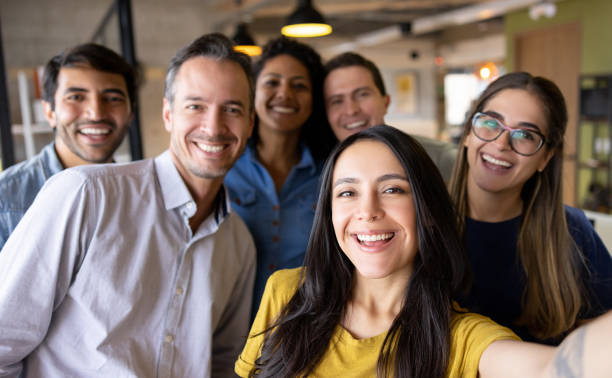
\includegraphics[width=0.6\textwidth]{foto-kelompok}\par

    % ---------- Disusun oleh ----------
    \vspace{1.2cm}
    {\bfseries Disusun oleh:\par}
    \vspace{0.2cm}
    \textbf{Muhammad Aufar Rizqi Kusuma}
    \vspace{0.5cm} \\

    % ---------- Institusi ----------
    \vspace{2.0cm}
    Laboratorium Ilmu dan Rekayasa Komputasi\par
    Program Studi Teknik Informatika\par
    Sekolah Teknik Elektro dan Informatika\par
    Institut Teknologi Bandung\par

\end{titlepage}

\clearpage
\pagestyle{fancy}

\tableofcontents
\clearpage

\chapter{Pendahuluan}
\section{Deskripsi Tugas}

Tugas kecil ini berfokus pada pembuatan \textit{solver} untuk permainan \textit{Ice Sliding Puzzle}. Program menerima sebuah papan permainan berbentuk $N \times M$ dari berkas teks, kemudian mencari urutan gerakan yang membawa pin dari posisi awal \texttt{Z} ke tujuan \texttt{O}. Selama pencarian, pin hanya dapat bergerak ke empat arah utama, dan karena lantai bersifat licin, pin akan terus meluncur sampai tertahan oleh dinding atau batu \texttt{X}.

Selain mencapai tujuan, solusi yang valid juga harus melewati angka-angka pada papan secara berurutan lengkap, mulai dari \texttt{0} hingga angka terbesar yang tersedia. Apabila pin melewati lava \texttt{L}, keluar dari batas papan, atau menginjak angka di luar urutan, maka keadaan tersebut dianggap gagal. Dengan demikian, program tidak hanya mencari jalur terpendek atau termurah, tetapi juga jalur yang mematuhi seluruh aturan permainan.

Gambar berikut memperlihatkan contoh papan permainan beserta legenda simbol yang digunakan pada laporan ini.

\begin{figure}[H]
    \centering
    \begin{tikzpicture}[
            x=1cm,
            y=1cm,
            board cell/.style={draw, line width=0.45pt, minimum size=1cm, inner sep=0pt, outer sep=0pt, align=center, font=\large\bfseries}
        ]
        \foreach \x/\y/\fillcolor/\value in {
                0/0/gray!10/*,
                1/0/yellow!25/0,
                2/0/gray!10/*,
                3/0/black!15/X,
                4/0/blue!20/O,
                0/1/gray!10/*,
                1/1/black!15/X,
                2/1/gray!10/*,
                3/1/gray!10/*,
                4/1/red!20/L,
                0/2/green!25/Z,
                1/2/gray!10/*,
                2/2/yellow!25/1,
                3/2/gray!10/*,
                4/2/gray!10/*,
                0/3/gray!10/*,
                1/3/gray!10/*,
                2/3/gray!10/*,
                3/3/black!15/X,
                4/3/gray!10/*
            } {
                \node[board cell, fill=\fillcolor] at (\x+0.5,3.5-\y) {\value};
            }
        \draw[line width=0.8pt] (0,0) rectangle (5,4);
    \end{tikzpicture}
    \caption{Contoh visualisasi papan \textit{Ice Sliding Puzzle}.}
    \label{fig:contoh-papan-ice-sliding}
\end{figure}

\noindent
Pada contoh di atas, simbol \texttt{Z} menandai posisi awal, \texttt{O} menandai tujuan, \texttt{X} adalah rintangan, \texttt{L} adalah lava, sedangkan \texttt{0} dan \texttt{1} adalah angka yang harus dilewati secara berurutan sebelum pin dapat dinyatakan menang. Tile bertanda \texttt{*} merepresentasikan jalur kosong yang dapat dilewati pin.

\section{Spesifikasi Program}
\begin{itemize}
    \item  Buatlah sebuah program tersebut dalam bahasa Java, Python, C++, C, atau GO yang mengimplementasikan algoritma Pathfinding (UCS, GBFS, dan A*) untuk mencari solusi dalam permainan Ice Sliding Puzzle Solver.
    \item Tugas dikerjakan berkelompok dengan anggota maksimal 2 orang, boleh lintas kelas maupun kampus. Silahkan isi pendataan kelompok pada link berikut.
    \item  \textbf{Input}: program akan memberikan pengguna sebuah arahan pada terminal (jika tidak mengerjakan bonus) untuk memilih file test case berekstensi .txt, kemudian program membaca file test case tersebut yang berisi konfigurasi awal dari map Permainan yang akan diselesaikan. Perhatikan bahwa input dapat memiliki ukuran papan yang berbeda-beda (tidak harus persegi), serta program harus dapat memvalidasi apakah input yang diberikan merupakan input valid atau bukan.
\end{itemize}

Contoh perhitungan cost gerakan adalah sebagai berikut.
\begin{itemize}
    \item Misalkan aktor melakukan satu gerakan ke kanan dan selama gerakan tersebut melewati tiga tile dengan cost berturut-turut: 2, 5, dan 4. Maka cost gerakan itu adalah $2 + 5 + 4 = 11$.
    \item Total cost solusi adalah jumlah dari semua cost gerakan yang dilakukan sepanjang solusi.
    \item Perlu diingat: tile `X` dan `L` tetap mempunyai nilai cost dalam input, tetapi tidak dihitung dalam solusi valid karena `X` tidak pernah dilewati dan `L` menyebabkan game over jika dilewati.
\end{itemize}

\begin{tcolorbox}[
        colback=black!3,
        colframe=black!60,
        boxrule=0.6pt,
        left=1mm,
        right=1mm,
        top=1mm,
        bottom=1mm,
        listing only,
        listing options={basicstyle=\ttfamily\small, columns=fullflexible, keepspaces=true}
    ]
    Contoh: \\
    Gerakan 1: tiles traversed costs = 2, 5, 4, maka movement cost = 11 \\
    Gerakan 2: tiles traversed costs = 3, 2, maka movement cost = 5 \\
    Total cost solusi = $11 + 5 = 16$
\end{tcolorbox}

\section{Output}

Program harus menghasilkan keluaran berikut setelah pencarian selesai:
\begin{enumerate}
    \item Menampilkan solusi gerakan yang ditemukan (mis. RULUDR...).
    \item Menampilkan total cost dari solusi.
    \item Menampilkan visualisasi papan pada solusi, yaitu keadaan papan sehingga aktor dapat mencapai titik \texttt{O} menggunakan algoritma pathfinding yang dipilih. Visualisasi ini harus menandai lintasan akhir yang ditempuh aktor.
    \item Menampilkan jumlah konfigurasi / iterasi yang ditinjau oleh algoritma. Program harus menyediakan opsi untuk menyimpan setiap iterasi (state) ke file berekstensi \texttt{.txt} sehingga dapat dianalisis atau diputar ulang nanti.
    \item Menampilkan waktu eksekusi algoritma dalam milidetik. Pengukuran waktu harus meliputi hanya waktu komputasi (search), tidak termasuk waktu I/O membaca/menulis file.
    \item Playback (bukan live update), dimana setelah algoritma selesai, program harus dapat memvisualisasikan proses pathfinding sebagai rangkaian langkah yang dapat diputar mundur/maju. Contoh playback di CLI dapat berisi fitur-fitur di bawah ini.
          \begin{enumerate}
              \item Arrow kiri/kanan untuk mundur/maju satu step.
              \item ESC: prompt user untuk memasukkan nomor step X dan langsung lompat ke step tersebut.
          \end{enumerate}
\end{enumerate}

Catatan: untuk mode GUI (bonus), playback harus memiliki kontrol kecepatan (play/pause/seek) dan kemampuan maju/mundur yang setara dengan pengalaman video. Berikut adalah contoh file .txt yang akan dijadikan sebagai input.
\\ \\
Baris pertama memuat 2 angka $(N, M)$ yang menyatakan panjang dan lebar papan \\
N baris berikutnya merepresentasikan papan \\
N baris berikutnya merepresentasikan cost untuk melewati tile tersebut \\

\begin{tcolorbox}[
        title=Contoh Input,
        listing only,
        enhanced,
        sharp corners,
        colback=black!2,
        colframe=black!70,
        boxrule=0.7pt,
        fonttitle=\bfseries\small,
        left=2mm,
        right=2mm,
        top=1mm,
        bottom=1mm,
        listing options={basicstyle=\ttfamily\footnotesize, columns=fullflexible, keepspaces=true, breaklines=false, showstringspaces=false, showtabs=false, tabsize=2}
    ]
    7 7 \\
    XXXXXXX \\
    X0****X \\
    X**X**X \\
    X****OX \\
    X***1LX \\
    XZ**X*X \\
    XXXXXXX \\
    999 999 999 999 999 999 999 \\
    999 3 5 2 8 1 999 \\
    999 7 4 999 6 9 999 \\
    999 2 8 3 5 4 999 \\
    999 6 1 7 2 999 999 \\
    999 9 3 4 999 8 999 \\
    999 999 999 999 999 999 999 \\
\end{tcolorbox}

\noindent
Keterangan:
\begin{itemize}
    \item \texttt{*} = path yang bisa dilewati.
    \item \texttt{X} = Rintangan/Batu. Aktor akan berhenti tepat sebelum batu.
    \item \texttt{L} = Lava. Melewati lava akan mengalami game over (meskipun tidak berhenti tepat di lava).
    \item \texttt{Z} = Aktor/Pengguna.
    \item \texttt{O} = Titik tujuan.
    \item \texttt{<i>} = Angka. Ini adalah modifikasi pada spesifikasi tugas. Aktor harus melewati angka-angka ini sesuai urutan yang ada pada papan. Petak berangka 1 harus dilewati setelah aktor melewati petak berangka 0. petak berangka 2 harus dilewati setelah petak berangka 1 dan seterusnya (maksimal sampai 9).
\end{itemize}

\noindent
Aturan tambahan yang penting.
\begin{itemize}
    \item Jika aktor menginjak angka di luar urutan (mis.\, menginjak 1 sebelum 0), maka kondisi tersebut dianggap game over.
    \item Setelah sebuah petak angka dilewati sesuai urutan, petak tersebut berubah menjadi petak biasa dan dapat dilalui lagi tanpa batasan urutan.
    \item Petak angka adalah tile normal (bukan rintangan). Akibatnya, aktor akan meluncur melewatinya jika bergerak tanpa berhenti.
    \item Jika aktor bergerak menuju sisi papan (kanan/atas/kiri/bawah) dan tidak ada rintangan pada sisi tersebut untuk menghentikannya, maka aktor akan keluar papan dan kondisi dianggap game over. Dengan demikian, permainan harus diulang dari awal.
    \item Pin/aktor harus tepat berhenti pada titik \texttt{O} dan semua angka harus telah dilewati sesuai urutan agar kondisi dianggap sukses.
    \item Setiap tile memiliki cost traversal yang diberikan pada bagian kedua input. Cost merepresentasikan biaya ketika aktor melewati suatu tile.
    \item Cost gerakan dihitung dari jumlah cost seluruh tile yang dilalui selama satu gerakan sliding. Tile posisi awal pada awal gerakan tidak dihitung, tetapi tile tempat aktor berhenti pada akhir gerakan tetap dihitung.
\end{itemize}

\section{Spesifikasi Bonus}

Poin maksimal untuk bonus adalah 10. Mahasiswa dapat memilih satu atau beberapa spesifikasi bonus di bawah ini; total poin tambahan yang diberikan untuk tugas tidak boleh melebihi 10 poin.

\begin{enumerate}
    \item \textbf{GUI penuh untuk program (maks 6 poin)}. Membuat antarmuka grafis yang memungkinkan pengguna memilih file input, menampilkan papan, mengatur kecepatan playback, dan memutar langkah mundur/maju. Kriteria penilaian:

    \item \textbf{Tambahkan algoritma pathfinding tambahan (maks 2 poin)}. Implementasi setidaknya satu algoritma pathfinding lain selain yang diwajibkan (mis.\, Dijkstra, IDA*, BFS adaptif untuk sliding puzzle, atau algoritma lain yang relevan). Penilaian:

    \item \textbf{Tambahkan dua alternatif heuristik (maks 2 poin)}. Sediakan dua heuristik tambahan untuk A* selain heuristik utama. Kriteria:

    \item \textbf{Optimasi kecepatan pencarian (maks 5 poin, tetapi total bonus tetap dibatasi)}. Optimasi yang dapat meningkatkan kecepatan menemukan solusi. Penilaian didasarkan pada bukti eksperimen dan metrik yang jelas.
\end{enumerate}

Catatan penting tentang pemberian nilai.
\begin{itemize}
    \item Total poin bonus yang diberikan tidak boleh melebihi 10, meskipun jumlah maksimum per-item jika dijumlahkan lebih besar. Dosen/TA akan memilih kombinasi fitur yang memberi nilai maksimal hingga 10 poin.
    \item Untuk setiap fitur bonus, sertakan bukti fungsionalitas: screenshot GUI atau rekaman pendek (untuk GUI), hasil benchmark (untuk kecepatan), dan contoh keluaran atau log yang menunjukkan algoritma/heuristik baru bekerja.
    \item Semua kode bonus harus disertakan pada repositori akhir dan dilengkapi instruksi build/run di README.
\end{itemize}

Instruksi pengumpulan bonus.
\begin{itemize}
    \item Sertakan penjelasan singkat di README tentang fitur bonus yang diimplementasikan dan bagaimana mengaktifkannya (mis.\, argumen CLI atau flag pada GUI).
    \item Apabila mengumpulkan GUI, sertakan screenshot dan langkah untuk menjalankan (dependensi, command build, dan cara membuka file input).
\end{itemize}



\chapter{Algoritma Penyelesaian}
\section{Algoritma Uniform Cost Search (UCS)}

Uniform Cost Search (UCS) adalah algoritma pencarian yang mengembangkan node dengan biaya jalur terkecil $g(n)$ terlebih dahulu. UCS menjamin menemukan solusi dengan total biaya minimum apabila semua biaya tepi bernilai tidak negatif, karena selalu memilih state dengan $g$ terkecil untuk diekspansi \cite{dijkstra1959note,russell2010artificial}. Beberapa sifat penting UCS adalah sebagai berikut.
\begin{itemize}
    \item \textbf{Optimalitas}. UCS optimal jika biaya tiap langkah non-negatif.
    \item \textbf{Keterlengkapan}. UCS akan menemukan solusi apabila ruang status berhingga dan ada path menuju tujuan.
    \item \textbf{Kompleksitas}. Bergantung pada branching factor dan distribusi biaya. Pada kasus terburuk dapat menimbulkan eksplorasi besar jika banyak node memiliki biaya jalur serupa.
\end{itemize}

\subsection{Definisi $f(n)$ dan $g(n)$ untuk UCS}
Dalam implementasi solver Ice Sliding Puzzle ini, definisi fungsi biaya yang digunakan adalah sebagai berikut.
\begin{itemize}
    \item $g(n)$: total biaya kumulatif dari semua gerakan yang dilakukan dari keadaan awal sampai mencapai node/state $n$. Untuk setiap gerakan sliding, biaya gerakan adalah jumlah cost dari tiap tile yang dilalui selama sliding (catatan: tile posisi awal sebelum sliding tidak dihitung, tetapi tile tempat aktor berhenti dihitung).
    \item $f(n)$: untuk UCS, kita menggunakan $f(n)=g(n)$. Prioritas antrian eksplorasi didasarkan pada nilai $g(n)$ terkecil.
\end{itemize}

\subsection{Implementasi UCS pada Kode Sumber}
Berdasarkan implementasi di \texttt{src/core/search/Search.cpp}, UCS dijalankan melalui fungsi umum \texttt{Search::solve} dengan aturan prioritas \texttt{computePriority = gCost}. State direpresentasikan sebagai triple \texttt{(row, col, nextCheckpoint)}. Di bawah ini adalah uraian langkah demi langkah yang merepresentasikan apa yang dilakukan kode pada setiap tahap.

\begin{enumerate}
    \item \textbf{Inisialisasi state awal}: buat node awal dengan posisi start, \texttt{nextCheckpoint=0}, \texttt{g=0}, dan hitung heuristik (meskipun untuk UCS heuristik tidak dipakai untuk prioritas, nilai h biasanya disimpan untuk konsistensi struktur node).
    \item \textbf{Siapkan frontier}: buat \texttt{priority\_queue} (disebut \texttt{frontier}) yang mengurutkan node menurut prioritas; untuk UCS prioritas ini adalah \texttt{gCost}.
    \item \textbf{Best-cost map}: buat \texttt{unordered\_map<StateKey,int>} bernama \texttt{bestCost} untuk menyimpan biaya terbaik (terkecil) yang pernah ditemukan untuk setiap state (key = posisi + nextCheckpoint).
    \item \textbf{Masukkan start}: push node awal ke \texttt{frontier} dan set \texttt{bestCost[start.state] = 0}.
    \item \textbf{Main loop}: selama \texttt{frontier} tidak kosong, ambil node dengan prioritas terkecil (pop): ini adalah node dengan \texttt{g} terkecil pada saat itu.
    \item \textbf{Pruning cepat}: jika node yang di-pop memiliki \texttt{g > bestCost[state]} berarti ada jalur lebih baik yang sudah dicatat -> lewati node tersebut (continue).
    \item \textbf{Cek goal}: periksa apakah node memenuhi kondisi goal (posisi = goal dan \texttt{nextCheckpoint > maxCheckpoint}). Jika ya, lakukan rekonstruksi jalur (backtrack menggunakan \texttt{parentIndex}) dan kembalikan hasil.
    \item \textbf{Generate successor}: untuk setiap arah gerak (Up/Down/Left/Right) panggil \texttt{rules.applyMove(board, current.pos, current.nextCheckpoint, dir)}. Fungsi ini meng-"slide" aktor sampai berhenti, mengakumulasi biaya tile yang dilalui, dan mengembalikan posisi akhir, biaya gerak serta nilai \texttt{nextCheckpoint} baru bila melewati checkpoint.
    \item \textbf{Filter outcome tidak valid}: jika hasil \texttt{applyMove} menyatakan \texttt{outOfBounds}, \texttt{hitLava}, atau gerakan invalid lainnya, abaikan successor tersebut.
    \item \textbf{Hitung biaya kumulatif}: untuk setiap successor valid, hitung \texttt{next.g = current.g + outcome.moveCost} dan bentuk \texttt{next.state = (outcome.end, outcome.nextCheckpoint)}.
    \item \textbf{Pruning berdasarkan bestCost}: jika \texttt{bestCost[next.state]} ada dan \texttt{next.g >= bestCost[next.state]}, abaikan successor (jalur lebih mahal atau sama sudah ada). Jika lebih baik, set \texttt{bestCost[next.state] = next.g}.
    \item \textbf{Enqueue}: masukkan successor ke \texttt{frontier} dengan prioritas \texttt{next.g}. Simpan indeks parent untuk rekonstruksi jalur.
\end{enumerate}

\begin{algorithm}[H]
    \caption{Uniform Cost Search (UCS) pada Solver}
    \begin{algorithmic}[1]
        \Require \textit{board}, \textit{rules}
        \Ensure \textit{SearchResult}
        \State $start \gets (board.start, nextCheckpoint=0, g=0)$
        \State $frontier \gets$ priority queue terurut naik berdasarkan $g$
        \State masukkan $start$ ke $frontier$
        \State $bestCost[(start.pos, start.nextCheckpoint)] \gets 0$
        \While{$frontier$ tidak kosong}
        \State $current \gets pop(frontier)$
        \If{$current.g > bestCost[current.state]$}
        \State \textbf{continue}
        \EndIf
        \If{$isGoalState(current.pos, current.nextCheckpoint)$}
        \State \Return $reconstructPath(current)$
        \EndIf
        \For{setiap $dir \in \{Up, Down, Left, Right\}$}
        \State $outcome \gets applyMove(board, current.pos, current.nextCheckpoint, dir)$
        \If{$outcome.invalid$ \textbf{or} $outcome.hitLava$ \textbf{or} $outcome.outOfBounds$}
        \State \textbf{continue}
        \EndIf
        \State $next.g \gets current.g + outcome.moveCost$
        \State $next.state \gets (outcome.end, outcome.nextCheckpoint)$
        \If{$outcome.end = board.goal$ \textbf{and} $outcome.nextCheckpoint \le board.maxCheckpoint$}
        \State \textbf{continue}
        \EndIf
        \If{$next.state \in bestCost$ \textbf{and} $next.g \ge bestCost[next.state]$}
        \State \textbf{continue}
        \EndIf
        \State $bestCost[next.state] \gets next.g$
        \State masukkan $next$ ke $frontier$ dengan prioritas $next.g$
        \EndFor
        \EndWhile
        \State \Return \textit{failure}
    \end{algorithmic}
\end{algorithm}

\subsection{Contoh Pencarian UCS}
Sebagai ilustrasi, misalkan terdapat graf pencarian sederhana berikut. Angka di dalam kurung menunjukkan biaya kumulatif $g(n)$.

\begin{figure}[H]
    \centering
    \begin{tikzpicture}[
            level distance=14mm,
            sibling distance=28mm,
            every node/.style={draw, circle, minimum size=7mm, inner sep=0pt},
            chosen/.style={draw, circle, fill=gray!25, minimum size=7mm, inner sep=0pt},
            edge from parent/.style={draw, -latex}
        ]
        \node[draw, rectangle, rounded corners, fill=gray!10] (S) {$S(0)$}
        child { node[draw, rectangle, rounded corners, fill=gray!10] (A) {$A(2)$}
                child { node[draw, rectangle, rounded corners, fill=gray!10] (D) {$D(5)$}
                        child { node[chosen] (G1) {$G(8)$} }
                    }
            }
        child { node[draw, rectangle, rounded corners, fill=gray!10] (B) {$B(1)$}
                child { node[draw, rectangle, rounded corners, fill=gray!10] (C) {$C(4)$}
                        child { node[chosen] (G2) {$G(9)$} }
                    }
            };
        \draw[very thick, blue] (S) -- (A) -- (D) -- (G1);
    \end{tikzpicture}
    \caption{Contoh pohon pencarian UCS. Jalur terpilih adalah $S \rightarrow A \rightarrow D \rightarrow G$ karena memiliki biaya kumulatif minimum pada setiap ekspansi.}
    \label{fig:contoh-ucs}
\end{figure}

Pada contoh ini, urutan rute yang dipilih adalah $S \rightarrow A \rightarrow D \rightarrow G$. UCS selalu memilih node dengan $g(n)$ terkecil, sehingga meskipun ada cabang lain yang tampak lebih pendek secara langkah, jalur dengan biaya kumulatif paling kecil tetap diprioritaskan.

\section{Algoritma Greedy Best-First Search (GBFS)}

Greedy Best-First Search (GBFS) merupakan algoritma pencarian yang memilih node untuk diekspansi berdasarkan nilai heuristik $h(n)$ saja, yakni node yang dianggap paling "dekat" ke tujuan menurut heuristik. GBFS tidak mempertimbangkan biaya jalur $g(n)$ sehingga dapat menjadi sangat cepat namun tidak menjamin optimalitas atau keterlengkapan dalam semua kasus \cite{russell2010artificial}. Karakteristik GBFS dapat dijabarkan sebagai berikut.
\begin{itemize}
    \item \textbf{Kecepatan}. Seringkali lebih cepat menemukan solusi dibanding pencarian yang mempertimbangkan $g(n)$, terutama bila heuristik sangat informatif.
    \item \textbf{Non-optimal}. GBFS tidak menjamin menemukan solusi dengan biaya minimal.
    \item \textbf{Sensitif terhadap heuristik}. kualitas heuristik sangat menentukan performa dan hasil pencarian.
\end{itemize}

\subsection{Definisi $f(n)$ dan $g(n)$ untuk GBFS}
Untuk GBFS pada solver ini berlaku
\begin{itemize}
    \item $g(n)$: sama seperti pada UCS, dapat dihitung sebagai total biaya kumulatif sampai node $n$, namun nilai ini \emph{tidak} digunakan untuk menentukan urutan ekspansi.
    \item $f(n)$: GBFS menggunakan $f(n)=h(n)$, yaitu hanya mengurutkan node menurut estimasi heuristik menuju tujuan. Dengan demikian antrian prioritas berdasarkan $h(n)$ saja.
\end{itemize}

\subsection{Implementasi GBFS pada Kode Sumber}
Pada kode sumber yang sama, GBFS tidak membuat fungsi terpisah; perbedaannya hanya pada prioritas antrian: \texttt{computePriority = hCost}. Nilai heuristik dihitung oleh \texttt{Heuristic::estimate} (\texttt{src/core/heuristic/Heuristic.cpp}) sesuai pilihan \texttt{HeuristicType}. Di bawah ini alur langkah demi langkah implementasi GBFS dalam kode.

\begin{enumerate}
    \item \textbf{Inisialisasi}: buat node awal dengan \texttt{g=0} dan hitung \texttt{h = Heuristic::estimate(...)} untuk posisi awal.
    \item \textbf{Frontier}: buat \texttt{priority\_queue} yang mengurutkan node berdasarkan nilai heuristik \texttt{h} (nilai lebih kecil = prioritas lebih tinggi).
    \item \textbf{Best-cost map}: seperti UCS, tetap gunakan \texttt{bestCost} untuk menyimpan \texttt{g} terbaik yang ditemukan untuk setiap state. Ini membantu menghindari revisits yang jelas lebih mahal.
    \item \textbf{Masukkan start}: push node awal ke frontier dengan prioritas \texttt{start.h}.
    \item \textbf{Main loop}: pop node dengan \texttt{h} terkecil.
    \item \textbf{Pruning}: jika \texttt{current.g > bestCost[current.state]} maka lewati.
    \item \textbf{Cek goal}: jika memenuhi kondisi goal, rekonstruksi dan kembalikan jalur.
    \item \textbf{Generate successor}: untuk tiap arah, panggil \texttt{rules.applyMove} untuk mendapatkan posisi akhir dan \texttt{moveCost} sama seperti pada UCS.
    \item \textbf{Validasi}: tolak successor yang outOfBounds, hitLava, atau invalid.
    \item \textbf{Kalkulasi g dan h}: hitung \texttt{next.g = current.g + outcome.moveCost} dan \texttt{next.h = Heuristic::estimate(..., outcome.end, outcome.nextCheckpoint)}.
    \item \textbf{Pruning bestCost}: jika ada entri \texttt{bestCost[next.state]} yang lebih baik, abaikan; jika lebih baik, perbarui \texttt{bestCost[next.state] = next.g}.
    \item \textbf{Enqueue}: push successor ke frontier dengan prioritas \texttt{next.h}. Simpan parent index untuk rekonstruksi.
\end{enumerate}

Catatan implementasi khusus GBFS di kode:
\begin{itemize}
    \item Meski prioritas adalah heuristik, penyimpanan \texttt{g} dan penggunaan \texttt{bestCost} membantu menghindari eksplorasi ulang yang jelas lebih mahal.
    \item Performa sangat bergantung pada kualitas heuristik: heuristik yang informatif mengarahkan eksplorasi ke goal dengan cepat.
\end{itemize}

\begin{algorithm}[H]
    \caption{Greedy Best-First Search (GBFS) pada Solver}
    \begin{algorithmic}[1]
        \Require \textit{board}, \textit{rules}, \textit{heuristicType}
        \Ensure \textit{SearchResult}
        \State $start.g \gets 0$
        \State $start.h \gets estimate(board, start.pos, start.nextCheckpoint, heuristicType)$
        \State $frontier \gets$ priority queue terurut naik berdasarkan $h$
        \State masukkan $start$ ke $frontier$ dengan prioritas $start.h$
        \State $bestCost[(start.pos, start.nextCheckpoint)] \gets 0$
        \While{$frontier$ tidak kosong}
        \State $current \gets pop(frontier)$
        \If{$current.g > bestCost[current.state]$}
        \State \textbf{continue}
        \EndIf
        \If{$isGoalState(current.pos, current.nextCheckpoint)$}
        \State \Return $reconstructPath(current)$
        \EndIf
        \For{setiap $dir \in \{Up, Down, Left, Right\}$}
        \State $outcome \gets applyMove(board, current.pos, current.nextCheckpoint, dir)$
        \If{$outcome.invalid$ \textbf{or} $outcome.hitLava$ \textbf{or} $outcome.outOfBounds$}
        \State \textbf{continue}
        \EndIf
        \State $next.g \gets current.g + outcome.moveCost$
        \State $next.h \gets estimate(board, outcome.end, outcome.nextCheckpoint, heuristicType)$
        \State $next.state \gets (outcome.end, outcome.nextCheckpoint)$
        \If{$outcome.end = board.goal$ \textbf{and} $outcome.nextCheckpoint \le board.maxCheckpoint$}
        \State \textbf{continue}
        \EndIf
        \If{$next.state \in bestCost$ \textbf{and} $next.g \ge bestCost[next.state]$}
        \State \textbf{continue}
        \EndIf
        \State $bestCost[next.state] \gets next.g$
        \State masukkan $next$ ke $frontier$ dengan prioritas $next.h$
        \EndFor
        \EndWhile
        \State \Return \textit{failure}
    \end{algorithmic}
\end{algorithm}

\subsection{Contoh Pencarian GBFS}
Misalkan heuristik yang digunakan memberi estimasi jarak ke tujuan seperti nilai di bawah ini. Angka dalam kurung adalah $h(n)$.

\begin{figure}[H]
    \centering
    \begin{tikzpicture}[
            level distance=14mm,
            sibling distance=28mm,
            every node/.style={draw, circle, minimum size=7mm, inner sep=0pt},
            chosen/.style={draw, circle, fill=gray!25, minimum size=7mm, inner sep=0pt},
            edge from parent/.style={draw, -latex}
        ]
        \node[draw, rectangle, rounded corners, fill=gray!10] (S) {$S(6)$}
        child { node[draw, rectangle, rounded corners, fill=gray!10] (A) {$A(4)$}
                child { node[chosen] (D) {$D(1)$}
                        child { node[chosen] (G1) {$G(0)$} }
                    }
            }
        child { node[draw, rectangle, rounded corners, fill=gray!10] (B) {$B(2)$}
                child { node[draw, rectangle, rounded corners, fill=gray!10] (C) {$C(3)$}
                        child { node[chosen] (G2) {$G(0)$} }
                    }
            };
        \draw[very thick, blue] (S) -- (B) -- (C) -- (G2);
    \end{tikzpicture}
    \caption{Contoh pohon pencarian GBFS. Jalur terpilih adalah $S \rightarrow B \rightarrow C \rightarrow G$ karena node-node pada cabang ini memiliki nilai heuristik paling kecil.}
    \label{fig:contoh-gbfs}
\end{figure}

Pada contoh ini, GBFS memilih node dengan nilai heuristik terkecil terlebih dahulu, sehingga jalur yang diambil tidak selalu jalur termurah. Fokus utamanya adalah mendekati tujuan secepat mungkin menurut estimasi heuristik.

\section{Algoritma A$^\ast$}

A$^\ast$ (A-star) merupakan algoritma \textit{Pathfinding} yang menggabungkan keuntungan UCS dan heuristik dengan menggunakan fungsi evaluasi
$$f(n) = g(n) + h(n),$$

untuk melakukan memilih path dengan cost paling minumum. Dalam hal ini, $g(n)$ adalah biaya jalur dari root ke node $n$ dan $h(n)$ adalah heuristik estimasi biaya dari $n$ ke tujuan. A$^\ast$ bersifat optimal jika heuristik $h$ adalah \emph{admissible} (tidak melebihkan cost sebenarnya) dan akan efisien apabila $h$ juga \emph{consistent} (monotonik) \cite{hart1968formal,russell2010artificial}. Sifat-sifat A$^\ast$ adalah sebagai berikut.
\begin{itemize}
    \item \textbf{Optimalitas}. Terjamin bila $h$ admissible.
    \item \textbf{Efisiensi}. Jumlah node yang diekspansi seminimal mungkin di antara semua algoritma yang menggunakan heuristik yang sama dan tetap optimal.
    \item \textbf{Ketergantungan heuristik}. Heuristik yang lebih informatif (mendekati nilai cost sebenarnya) akan mengurangi ruang pencarian.
\end{itemize}

\subsection{Definisi $f(n)$ dan $g(n)$ untuk A$^\ast$}
Pada A$^\ast$ yang diimplementasikan untuk Ice Sliding Puzzle adalah sebagai berikut.
\begin{itemize}
    \item $g(n)$: sama dengan UCS, total biaya kumulatif dari seluruh gerakan sampai node $n$, dengan tiap gerakan bernilai jumlah cost tile yang dilintasi selama sliding.
    \item $f(n)$: $f(n)=g(n)+h(n)$ di mana $h(n)$ adalah heuristik estimasi biaya tersisa. Untuk memastikan A$^\ast$ tetap optimal, pilih heuristik yang \emph{admissible}. Contoh heuristik admissible yang sering dipakai pada grid-based sliding problems adalah
          $$h(n) = d_{manhattan}(pos(n), goal) \times c_{min},$$
          di mana $d_{manhattan}$ adalah jarak Manhattan antara posisi berhenti aktor pada state $n$ dan posisi tujuan, dan $c_{min}$ adalah lower bound dari cost tiap tile pada instance (mis. nilai minimal dari matriks cost). Karena setiap langkah sliding setidaknya akan menempuh jarak fisik minimal dan setiap tile memiliki biaya tidak kurang dari $c_{min}$, heuristik ini tidak melebihkan biaya sebenarnya sehingga admissible.
\end{itemize}

\subsection{Implementasi A$^\ast$ pada Kode Sumber}
A$^\ast$ juga berbagi kerangka yang sama di \texttt{Search::solve}, tetapi prioritasnya menggunakan jumlah biaya aktual dan heuristik: \texttt{computePriority = gCost + hCost}. Di bawah ini langkah demi langkah yang persis tercermin di implementasi kode.

\begin{enumerate}
    \item \textbf{Inisialisasi node awal}: buat node awal dengan \texttt{g=0} dan hitung \texttt{h = Heuristic::estimate(...)} berdasarkan \texttt{HeuristicType} yang dipilih.
    \item \textbf{Frontier}: buat \texttt{priority\_queue} yang mengurutkan node berdasarkan nilai \texttt{f = g + h} (nilai lebih kecil = prioritas lebih tinggi). Comparator di kode juga menerapkan tie-breaker tambahan (mis. prioritas, lalu \texttt{gCost}, lalu urutan masuk) untuk determinisme.
    \item \textbf{Best-cost map}: buat atau gunakan \texttt{bestCost} untuk menyimpan \texttt{g} terbaik per state. Ini memastikan kita tidak memproses jalur yang jelas lebih mahal.
    \item \textbf{Masukkan start}: push node awal ke frontier dengan prioritas \texttt{start.g + start.h}.
    \item \textbf{Main loop}: pop node dengan fungsi evaluasi \texttt{f} terkecil.
    \item \textbf{Pruning cepat}: jika \texttt{current.g > bestCost[current.state]} lewati node.
    \item \textbf{Cek goal}: jika kondisi goal terpenuhi (posisi = goal dan semua checkpoint telah dilewati), rekonstruksi jalur dan kembalikan hasil.
    \item \textbf{Generate successor}: panggil \texttt{rules.applyMove} untuk tiap arah gerak. Fungsi ini memberikan posisi akhir, biaya gerak, dan update \texttt{nextCheckpoint} jika checkpoint dilintasi.
    \item \textbf{Validasi outcome}: abaikan successor jika \texttt{outcome.invalid}, \texttt{outcome.hitLava}, atau \texttt{outcome.outOfBounds}.
    \item \textbf{Kalkulasi g, h, f}: hitung \texttt{next.g = current.g + outcome.moveCost}, lalu \texttt{next.h = Heuristic::estimate(..., outcome.end, outcome.nextCheckpoint)}; prioritas yang akan dimasukkan adalah \texttt{next.f = next.g + next.h}.
    \item \textbf{Pruning bestCost}: jika sudah ada \texttt{bestCost[next.state]} dengan nilai lebih kecil atau sama, abaikan; jika lebih kecil, perbarui entry tersebut.
    \item \textbf{Enqueue}: push successor ke frontier dengan prioritas \texttt{next.f} dan simpan parent untuk rekonstruksi.
\end{enumerate}

Catatan implementasi penting:
\begin{itemize}
    \item \texttt{StateKey} yang memuat \texttt{nextCheckpoint} membuat posisi yang sama dengan progres berbeda menjadi state berbeda  ini penting untuk permasalahan checkpoint ordering.
    \item Pruning pada \texttt{bestCost} menggunakan \texttt{gCost} menjaga agar A$^\ast$ tidak memproses jalur yang lebih mahal menuju state yang sama, sekaligus kompatibel dengan heuristik admissible untuk memastikan optimalitas.
    \item Penentuan nilai heuristik (admissible vs.
          informed) menentukan apakah A$^\ast$ yang berjalan akan optimal dan seberapa efisien ia akan memotong ruang pencarian.
\end{itemize}

\begin{algorithm}[H]
    \caption{A* Search pada Solver}
    \begin{algorithmic}[1]
        \Require \textit{board}, \textit{rules}, \textit{heuristicType}
        \Ensure \textit{SearchResult}
        \State $start.g \gets 0$
        \State $start.h \gets estimate(board, start.pos, start.nextCheckpoint, heuristicType)$
        \State $frontier \gets$ priority queue terurut naik berdasarkan $(g+h)$
        \State masukkan $start$ ke $frontier$ dengan prioritas $start.g + start.h$
        \State $bestCost[(start.pos, start.nextCheckpoint)] \gets 0$
        \While{$frontier$ tidak kosong}
        \State $current \gets pop(frontier)$
        \If{$current.g > bestCost[current.state]$}
        \State \textbf{continue}
        \EndIf
        \If{$isGoalState(current.pos, current.nextCheckpoint)$}
        \State \Return $reconstructPath(current)$
        \EndIf
        \For{setiap $dir \in \{Up, Down, Left, Right\}$}
        \State $outcome \gets applyMove(board, current.pos, current.nextCheckpoint, dir)$
        \If{$outcome.invalid$ \textbf{or} $outcome.hitLava$ \textbf{or} $outcome.outOfBounds$}
        \State \textbf{continue}
        \EndIf
        \State $next.g \gets current.g + outcome.moveCost$
        \State $next.h \gets estimate(board, outcome.end, outcome.nextCheckpoint, heuristicType)$
        \State $next.state \gets (outcome.end, outcome.nextCheckpoint)$
        \If{$outcome.end = board.goal$ \textbf{and} $outcome.nextCheckpoint \le board.maxCheckpoint$}
        \State \textbf{continue}
        \EndIf
        \If{$next.state \in bestCost$ \textbf{and} $next.g \ge bestCost[next.state]$}
        \State \textbf{continue}
        \EndIf
        \State $bestCost[next.state] \gets next.g$
        \State masukkan $next$ ke $frontier$ dengan prioritas $next.g + next.h$
        \EndFor
        \EndWhile
        \State \Return \textit{failure}
    \end{algorithmic}
\end{algorithm}

\subsection{Admissibility pada A$^\ast$}
Secara teori, sebuah heuristik $h(n)$ disebut \emph{admissible} jika untuk setiap node $n$ berlaku
$$0 \le h(n) \le h^\ast(n),$$
dengan $h^\ast(n)$ adalah biaya minimum sebenarnya dari $n$ ke goal. Artinya, heuristik tidak boleh \emph{overestimate} biaya sisa. Jika A$^\ast$ menggunakan heuristik admissible, maka solusi pertama yang mencapai goal dijamin optimal \cite{hart1968formal,russell2010artificial}.

Selain admissible, sering dipakai juga syarat \emph{consistency} (monotonik), dimana
$$h(n) \le c(n,n') + h(n'),$$
untuk setiap transisi dari $n$ ke tetangga $n'$. Heuristik yang consistent selalu admissible, dan membuat nilai $f(n)$ tidak menurun sepanjang lintasan sehingga implementasi A$^\ast$ lebih stabil.


\subsection{Contoh Pencarian A$^\ast$}
Pada ilustrasi berikut, angka di dalam kurung menunjukkan nilai $f(n)=g(n)+h(n)$.

\begin{figure}[H]
    \centering
    \begin{tikzpicture}[
            level distance=14mm,
            sibling distance=28mm,
            every node/.style={draw, circle, minimum size=7mm, inner sep=0pt},
            chosen/.style={draw, circle, fill=gray!25, minimum size=7mm, inner sep=0pt},
            edge from parent/.style={draw, -latex}
        ]
        \node[draw, rectangle, rounded corners, fill=gray!10] (S) {$S(6)$}
        child { node[draw, rectangle, rounded corners, fill=gray!10] (A) {$A(5)$}
                child { node[chosen] (D) {$D(4)$}
                        child { node[chosen] (G1) {$G(5)$} }
                    }
            }
        child { node[draw, rectangle, rounded corners, fill=gray!10] (B) {$B(4)$}
                child { node[draw, rectangle, rounded corners, fill=gray!10] (C) {$C(4)$}
                        child { node[chosen] (G2) {$G(4)$} }
                    }
            };
        \draw[very thick, blue] (S) -- (B) -- (C) -- (G2);
    \end{tikzpicture}
    \caption{Contoh pohon pencarian A$^\ast$. Jalur terpilih adalah $S \rightarrow B \rightarrow C \rightarrow G$ karena kombinasi biaya aktual $g(n)$ dan heuristik $h(n)$ menghasilkan nilai $f(n)$ terkecil.}
    \label{fig:contoh-astar}
\end{figure}

Pada contoh ini, A$^\ast$ tidak hanya melihat kedekatan ke tujuan, tetapi juga biaya yang sudah ditempuh. Karena itu, jalur yang dipilih bisa berbeda dari GBFS dan lebih terarah menuju solusi optimal dibandingkan pencarian berbasis heuristik murni.

\section{Heuristik yang Digunakan}
Pada implementasi solver ini, tersedia beberapa heuristik yang dapat dipilih untuk dipakai pada algoritma A$^\ast$ maupun GBFS. Masing-masing heuristik dirancang untuk memberi estimasi jarak atau biaya yang berbeda terhadap posisi tujuan.

\begin{enumerate}
    \item \textbf{ManhattanToTarget}

          Heuristik ini menghitung jarak Manhattan dari posisi aktor saat ini ke titik tujuan \texttt{O}. Jika posisi aktor adalah $(x_1, y_1)$ dan tujuan berada pada $(x_2, y_2)$, maka
          $$h(n) = |x_1 - x_2| + |y_1 - y_2|.$$
          Heuristik ini sederhana dan cepat dihitung, sehingga cocok sebagai estimasi awal. Untuk A$^\ast$, nilai ini dapat dikalikan dengan biaya minimum tile agar lebih sesuai dengan fungsi cost.

    \item \textbf{RemainingPlusManhattan}

          Heuristik ini menggabungkan dua komponen, yaitu jumlah checkpoint/angka yang masih tersisa untuk dilewati dan jarak Manhattan ke target berikutnya. Secara intuitif, semakin banyak angka yang belum dilewati, semakin besar nilai heuristiknya. Bentuk sederhananya dapat ditulis sebagai
          $$h(n) = \alpha \cdot r(n) + \beta \cdot d_{manhattan}(pos(n), target(n)),$$
          dengan $r(n)$ adalah jumlah checkpoint yang tersisa, $target(n)$ adalah target yang harus dicapai berikutnya, dan $\alpha, \beta$ adalah bobot pengali.

    \item \textbf{WeightedRemainingToGoal}

          Heuristik ini memberi bobot lebih besar pada sisa checkpoint dan jarak menuju tujuan akhir. Dibandingkan heuristic sebelumnya, pendekatan ini lebih agresif karena mendorong pencarian untuk segera menyelesaikan urutan checkpoint sebelum fokus penuh ke tujuan akhir. Bentuk umumnya adalah
          $$h(n) = \gamma \cdot r(n) + \delta \cdot d_{manhattan}(pos(n), goal),$$
          dengan $\gamma$ dan $\delta$ sebagai bobot. Heuristik ini berguna jika ingin pencarian lebih terarah, tetapi perlu diuji agar tetap memberikan perilaku yang stabil pada berbagai papan.
\end{enumerate}

Secara umum, heuristik pertama lebih ringan dan sederhana, sedangkan dua heuristik lainnya mencoba memasukkan informasi progres permainan, yaitu jumlah checkpoint yang belum dilewati. Pemilihan heuristik bergantung pada tujuan pencarian, apakah lebih mengutamakan kecepatan komputasi, jumlah node yang diekspansi, atau kualitas solusi yang ditemukan.

\subsection{Admissibility Heuristik}
\begin{itemize}
    \item \textbf{ManhattanToTarget}: pada bentuk yang dipakai sebagai estimasi jarak murni, heuristik ini dapat dianggap \emph{admissible} selama ia hanya memberikan batas bawah terhadap biaya sisa. Dalam implementasi yang memperhitungkan cost tile, bentuk yang paling aman adalah $d_{manhattan}(pos(n), goal) \times c_{min}$, dengan $c_{min}$ sebagai cost tile terkecil pada papan. Jika hanya memakai Manhattan tanpa pengali cost minimum, heuristik tersebut tetap cenderung menjadi batas bawah pada jumlah langkah, tetapi belum tentu merepresentasikan batas bawah cost secara ketat pada papan dengan bobot tile yang bervariasi.

    \item \textbf{RemainingPlusManhattan}: heuristik ini \textbf{tidak dijamin admissible}. Alasannya, komponen jumlah checkpoint tersisa $r(n)$ dan bobot $\alpha, \beta$ dapat membuat estimasi lebih besar dari biaya sisa yang sebenarnya. Begitu heuristik mulai menambahkan penalti untuk checkpoint secara agresif, nilai $h(n)$ berpotensi melebihi cost minimum menuju solusi.

    \item \textbf{WeightedRemainingToGoal}: heuristik ini juga \textbf{tidak dijamin admissible}. Penggunaan bobot $\gamma$ dan $\delta$ membuat estimasi semakin fleksibel, tetapi sekaligus meningkatkan risiko overestimate. Heuristik ini lebih cocok dipakai sebagai heuristik \emph{informed} untuk mempercepat pencarian, bukan untuk menjamin optimalitas A$^\ast$.
\end{itemize}

Dengan demikian, jika tujuan utama adalah menjaga optimalitas A$^\ast$, heuristik yang paling aman dipakai adalah ManhattanToTarget dalam bentuk batas bawah cost. Sebaliknya, dua heuristik berbobot lebih cocok digunakan pada GBFS atau pada mode A$^\ast$ ketika optimalitas tidak menjadi prioritas utama.

\section{Komparasi Teoretis Algoritma Pencarian}

\subsection{Kriteria perbandingan}
Perbandingan didasarkan pada beberapa kriteria teoritis yang sering dipakai dalam analisis algoritma pencarian, yaitu
\begin{itemize}
    \item \textbf{Kompleksitas waktu}: jumlah node yang mungkin diekspansi sebagai fungsi branching factor $b$ dan kedalaman solusi $d$.
    \item \textbf{Kompleksitas memori}: ukuran frontier dan struktur data yang disimpan (sering menjadi batas praktis utama pada pencarian graf/ruang keadaan besar).
    \item \textbf{Kelengkapan (completeness)}: apakah algoritma menjamin menemukan solusi bila ada.
    \item \textbf{Optimalitas (optimality)}: apakah algoritma menjamin solusi biaya minimum menurut fungsi cost yang didefinisikan.
    \item \textbf{Ketergantungan pada heuristik}: bagaimana kualitas/jenis heuristik memengaruhi performa dan jaminan teori.
\end{itemize}

\subsection{Properti Algoritma}
\begin{itemize}
    \item \textbf{Uniform-Cost Search (UCS)}
          \begin{itemize}
              \item Kompleksitas waktu: dalam kasus terburuk, ekspansi bisa $O(b^{\lceil C^*/\epsilon\rceil})$ di mana $C^*$ adalah biaya solusi optimal dan $\epsilon$ adalah cost min positif pada edge; secara intuitif sangat sensitif terhadap rentang dan nilai cost.
              \item Kompleksitas memori: menyimpan seluruh frontier dan explored set (sering eksponensial pada $d$).
              \item Kelengkapan: lengkap jika semua edge cost $\ge 0$ dan graf tidak memuat siklus dengan cost negatif.
              \item Optimalitas: menjamin optimalitas biaya jika semua edge cost non-negatif.
              \item Heuristik: tidak memerlukan heuristik; tidak mendapat keuntungan dari informasi heuristik.
          \end{itemize}

    \item \textbf{Greedy Best-First Search (GBFS)}
          \begin{itemize}
              \item Kompleksitas waktu: sangat bergantung pada kualitas heuristik; dalam analisis kasar, dapat mendekati $O(b^d)$ jika heuristik menyesatkan, tetapi sering jauh lebih sedikit node diekspansi bila heuristik informatif.
              \item Kompleksitas memori: menyimpan frontier (biasanya lebih kecil dari UCS/A$^\ast$ pada kasus yang heuristiknya sangat informatif), tetapi masih bisa besar bila heuristik buruk.
              \item Kelengkapan: tidak selalu lengkap pada ruang keadaan dengan branching tak terbatas; pada graf finite biasanya lengkap jika implementasi menangani revisits, tetapi tidak ada jaminan teoretis umum.
              \item Optimalitas: tidak optimal  GBFS hanya mengejar nilai heuristik terkecil tanpa mempertimbangkan biaya yang sudah dikeluarkan.
              \item Heuristik: performa sangat sensitif terhadap akurasi heuristik; heuristik admissible/consistent tidak memberi jaminan optimalitas untuk GBFS.
          \end{itemize}

    \item \textbf{A$^\ast$}
          \begin{itemize}
              \item Kompleksitas waktu: secara teoretis antara UCS dan GBFS; node yang diekspansi bergantung pada seberapa informatif heuristik $h$. Semakin mendekati biaya sisa sebenarnya, semakin sedikit node yang diekspansi.
              \item Kompleksitas memori: menyimpan frontier dan explored set sama seperti UCS  bisa menjadi faktor pembatas utama.
              \item Kelengkapan: lengkap jika heuristic dan struktur graf memenuhi asumsi standar (mis. finite branching dan biaya edge non-negatif).
              \item Optimalitas: A$^\ast$ menjamin optimalitas jika heuristik \emph{admissible} (tidak overestimate) dan biasanya memerlukan konsistensi (monotonicity) agar implementasi dengan pruning sederhana tetap benar.
              \item Heuristik: kualitas heuristik menentukan efektivitas; heuristik admissible tapi lebih informatif (lebih tinggi namun dari cost sebenarnya) mengurangi ekspansi signifikan.
          \end{itemize}
\end{itemize}

\subsection{Perbandingan Teoretis}
\begin{itemize}
    \item \textbf{Admissibility vs. Konsistensi}: admissibility ($h(n) \le h^*(n)$) penting untuk optimalitas A$^\ast$. Konsistensi (monotonicity) memastikan bahwa nilai $f$ pada frontier tidak menurun dan memungkinkan implementasi tanpa perlu reprocessing node yang sudah diekspansi.

    \item \textbf{Pengaruh branching factor $b$ dan kedalaman $d$}: banyak analisis asymptotic didasarkan pada $b$ dan $d$. Ketika $b$ besar dan $d$ juga besar, biaya waktu dan memori tumbuh eksponensial sehingga teknik penghematan memori (IDA$^\ast$, search with limited memory) perlu dipertimbangkan.

    \item \textbf{Trade-off waktu vs memori}: UCS dan A$^\ast$ umumnya menukar memori untuk waktu (menyimpan frontier besar untuk menghindari rekalkulasi), sedangkan variasi seperti IDA$^\ast$ menurunkan memori dengan biaya waktu tambahan.

    \item \textbf{Kualitas heuristik}: heuristik yang lebih informatif (lebih dekat ke biaya sisa nyata) mengurangi jumlah node yang diekspansi, namun jika heuristik meng-overestimate (non-admissible), A$^\ast$ kehilangan jaminan optimalitas. GBFS memilih agresivitas heuristik di atas semua, sehingga sangat cepat bila heuristik akurat tetapi sangat berisiko bila heuristik menyesatkan.

\end{itemize}



\chapter{Implementasi}
\section{Arsitektur Program}

\section{Direktori Program}

\section{Modul-Modul Program}

\chapter{Eksperimen}
\section{Testing Kasus Dasar}
\begin{longtable}{c c c p{6cm}}
    \caption{Hasil eksperimen: input, output, dan deskripsi}\label{tab:eksperimen}                                                                                                                                                                                                             \\
    \hline
    No & Gambar Input                                                   & Gambar Output                                                   & Deskripsi                                                                                                                                          \\
    \hline
    \endfirsthead
    \multicolumn{4}{c}{{\bfseries \tablename\ \thetable{} -- lanjutan dari halaman sebelumnya}}                                                                                                                                                                                                \\
    \hline
    No & Gambar Input                                                   & Gambar Output                                                   & Deskripsi                                                                                                                                          \\
    \hline
    \endhead
    \hline \multicolumn{4}{r}{{Lanjutan pada halaman berikutnya}}                                                                                                                                                                                                                              \\
    \endfoot
    \hline
    \endlastfoot

    1  & 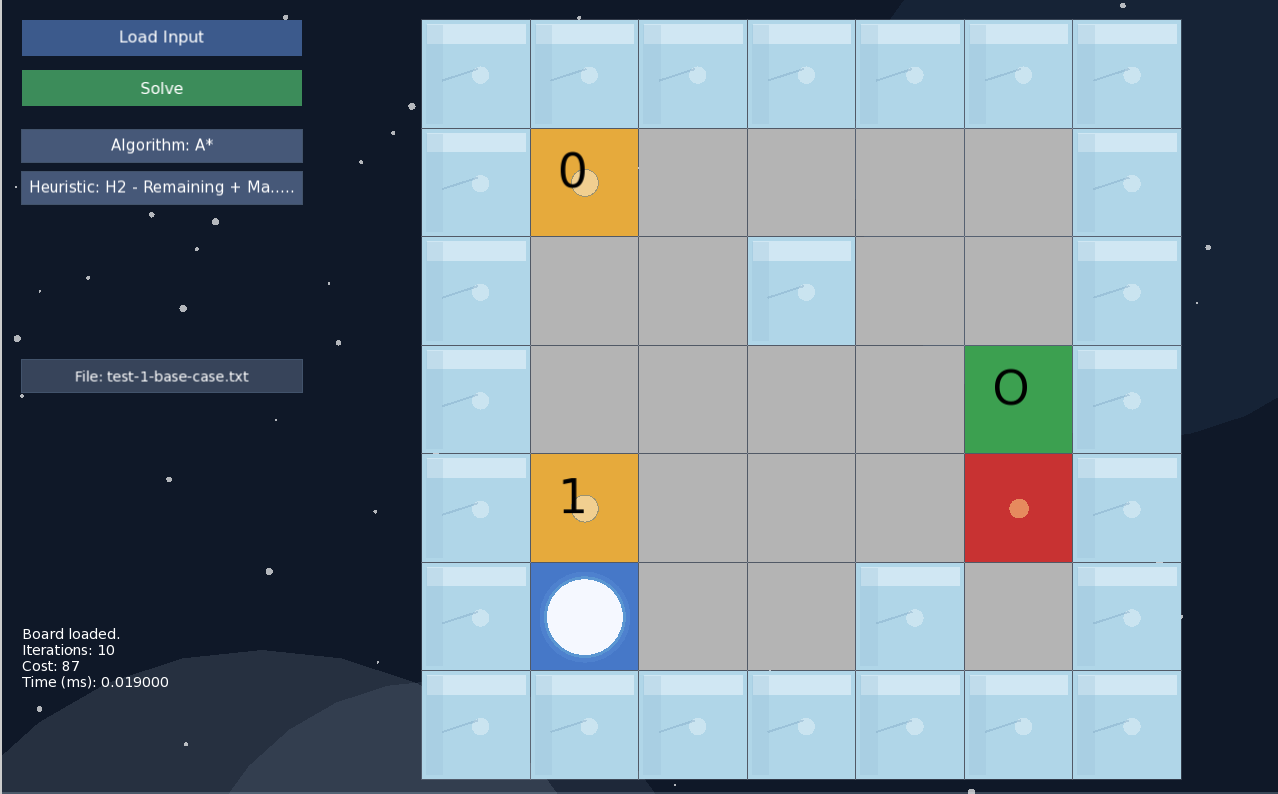
\includegraphics[width=0.25\linewidth]{04-eksperimen/in-1.png} & 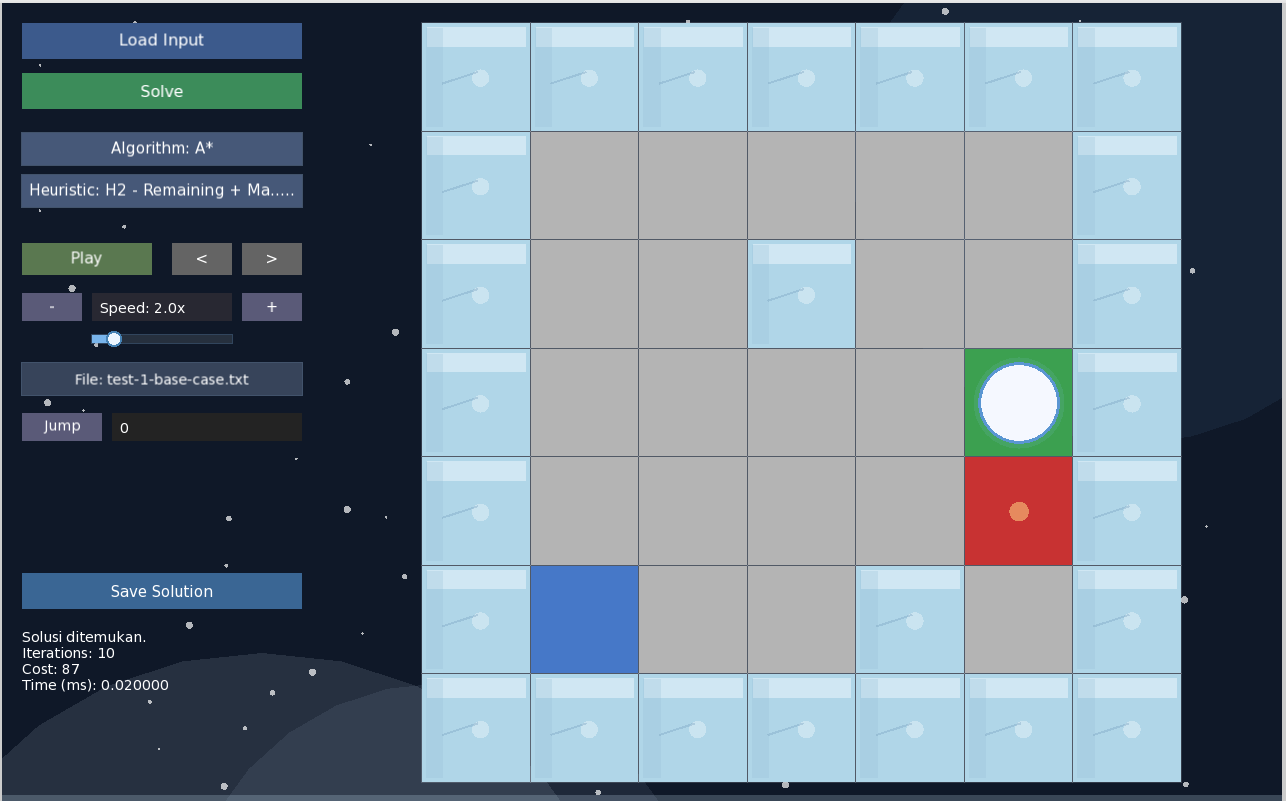
\includegraphics[width=0.25\linewidth]{04-eksperimen/out-1.png} & Test case pada ukuran $7 \times 7$ dengan Solusi Yang Ditemukan : \texttt{RULUDRUR} dan Cost dari Solusi : 87                                      \\
    2  & 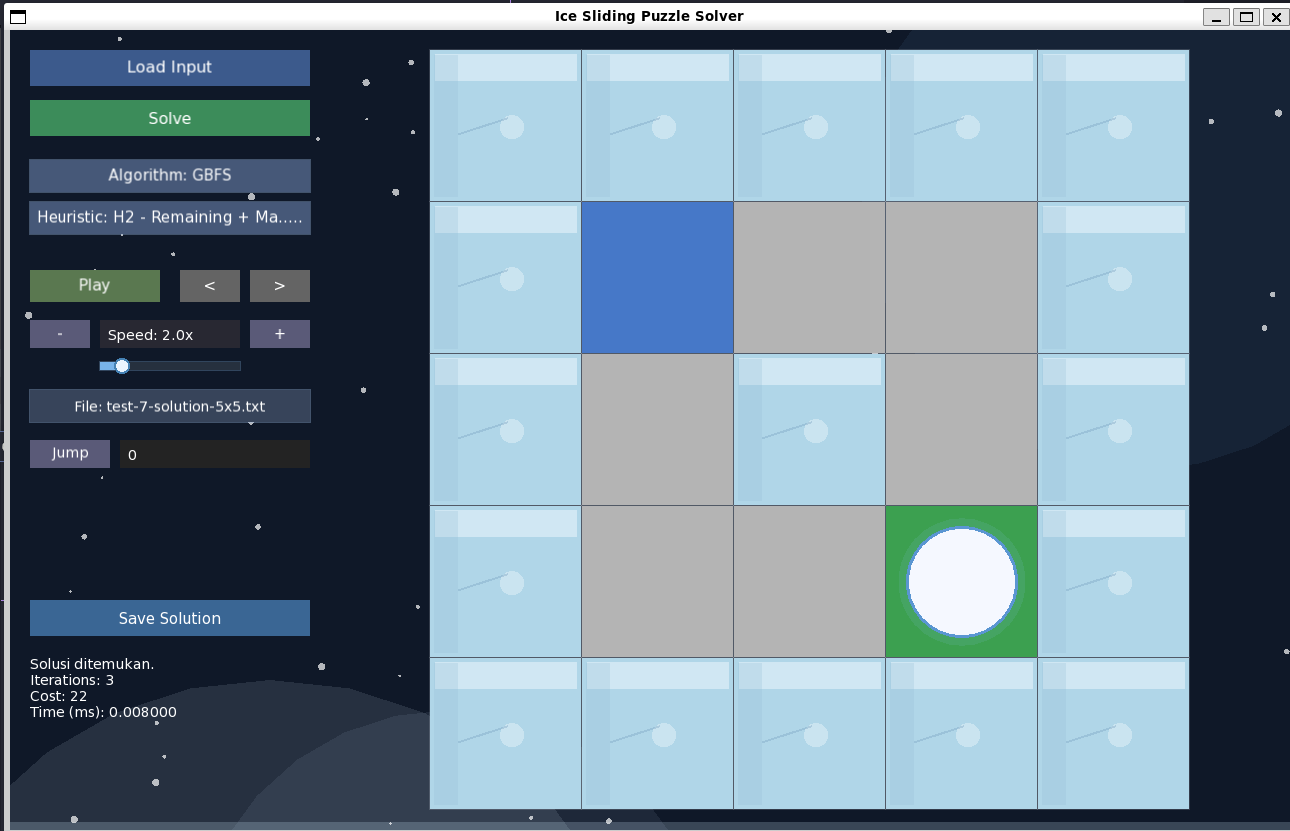
\includegraphics[width=0.25\linewidth]{04-eksperimen/in-2.png} & 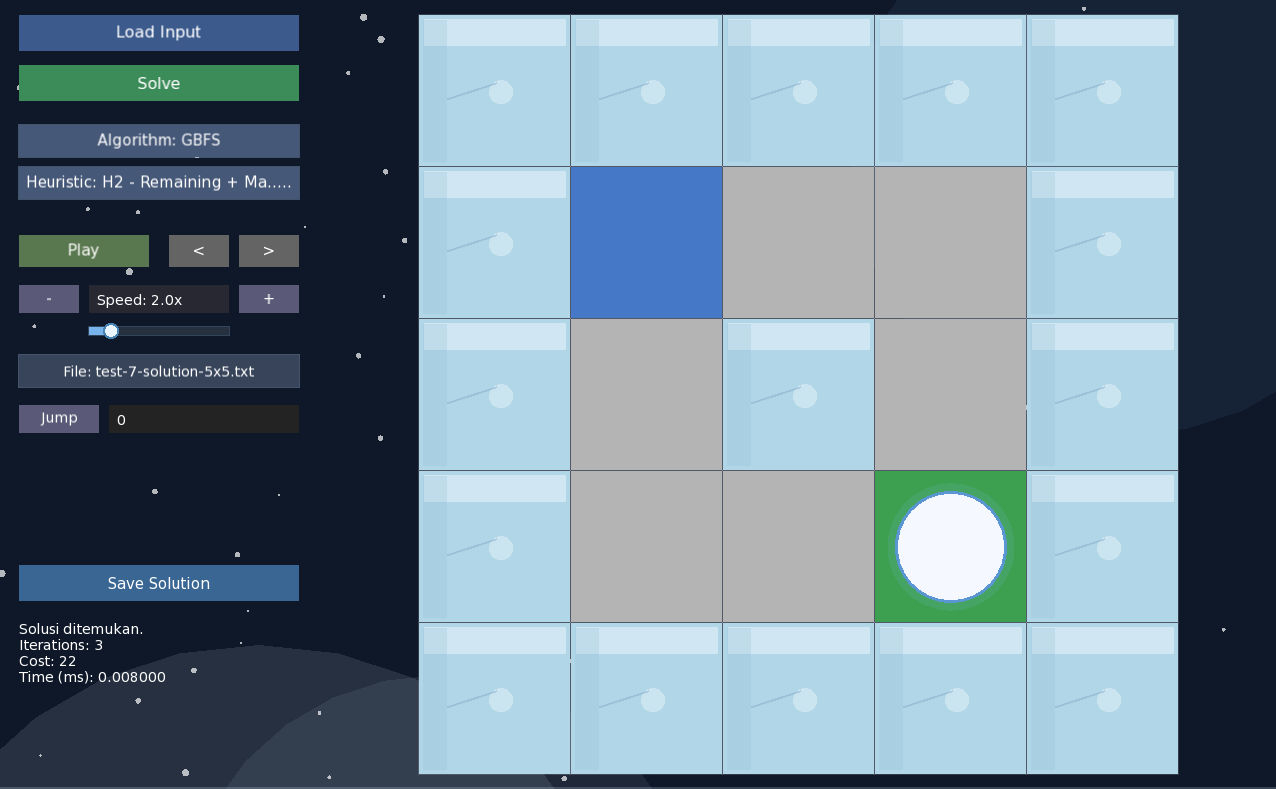
\includegraphics[width=0.25\linewidth]{04-eksperimen/out-2.png} & Test case dengan ukuran $ 5 \times 5$ dengan Solusi Yang Ditemukan : \texttt{DR} dan Cost dari Solusi : 22                                         \\
    3  & 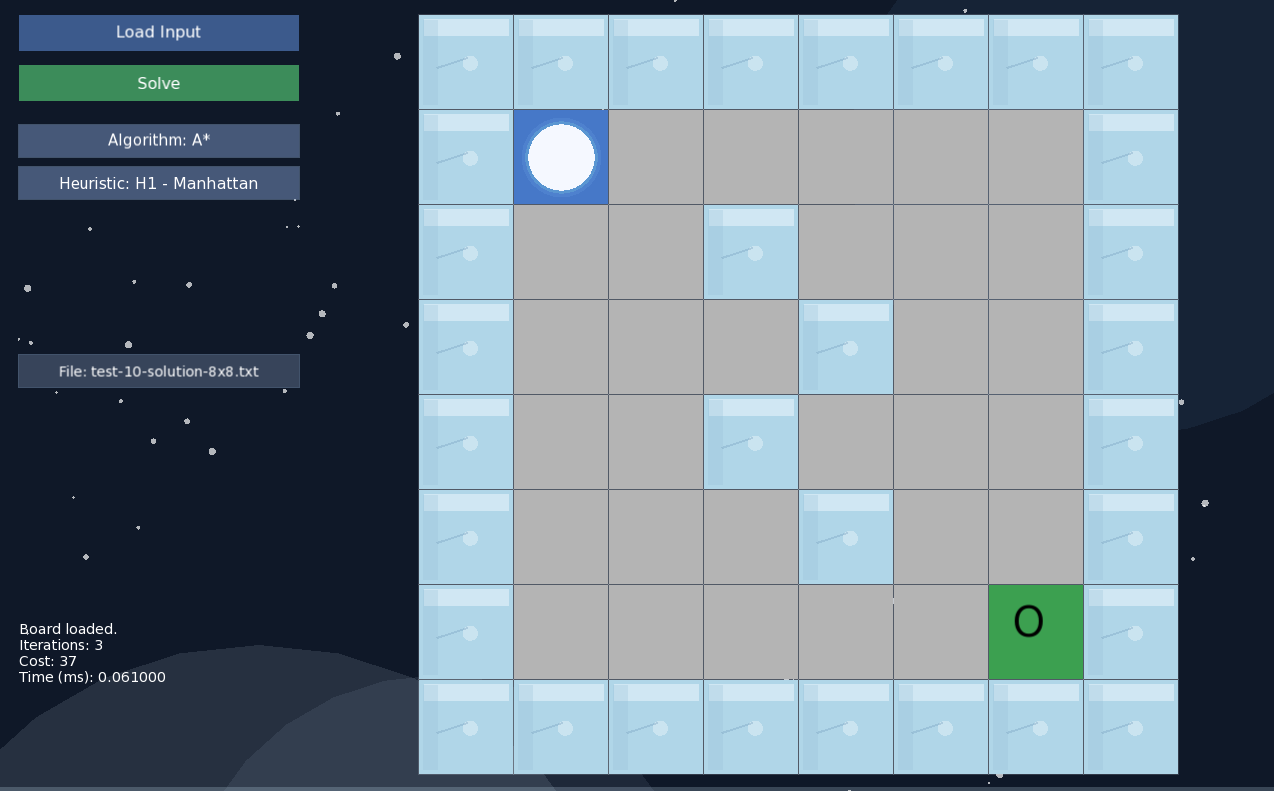
\includegraphics[width=0.25\linewidth]{04-eksperimen/in-3.png} & 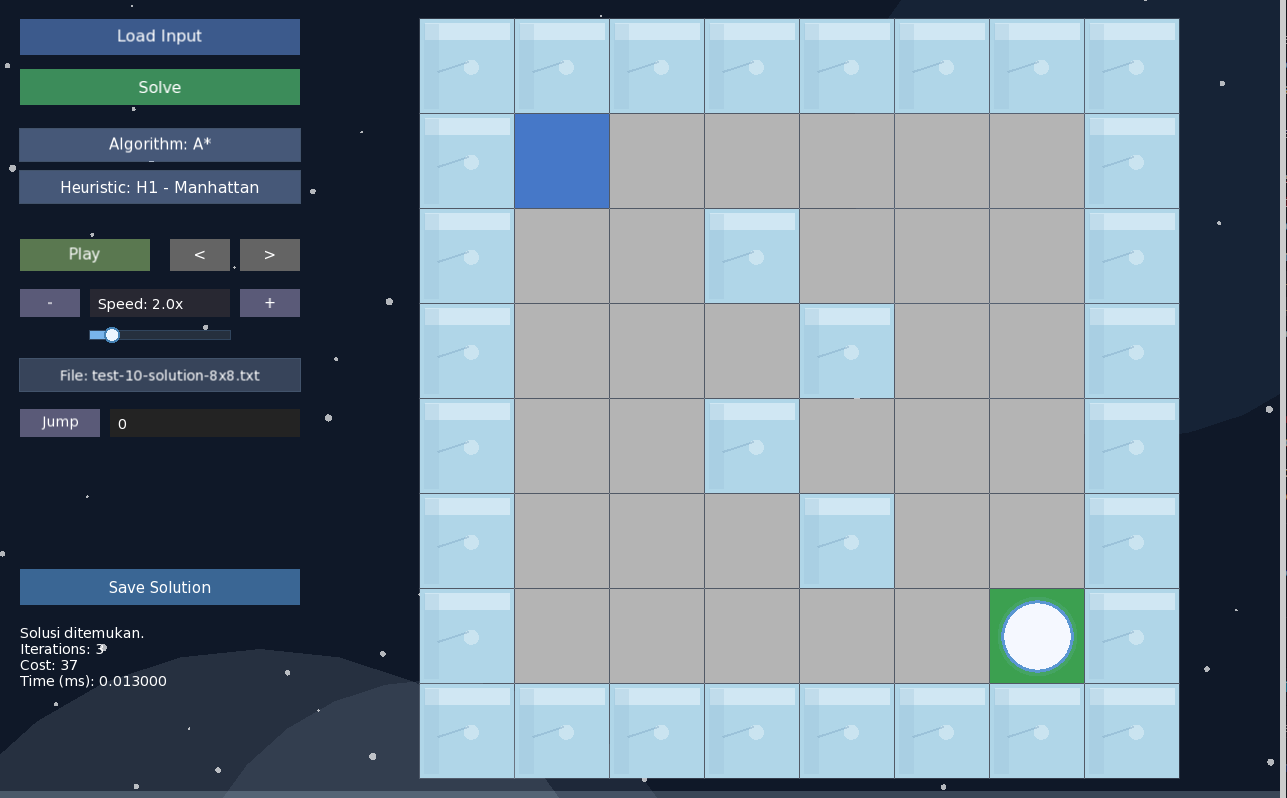
\includegraphics[width=0.25\linewidth]{04-eksperimen/out-3.png} & Test case dengan ukuran $8 \times 8$ dengan Solusi Yang Ditemukan : \texttt{RD} dan Cost dari Solusi : 37                                          \\

    4  & 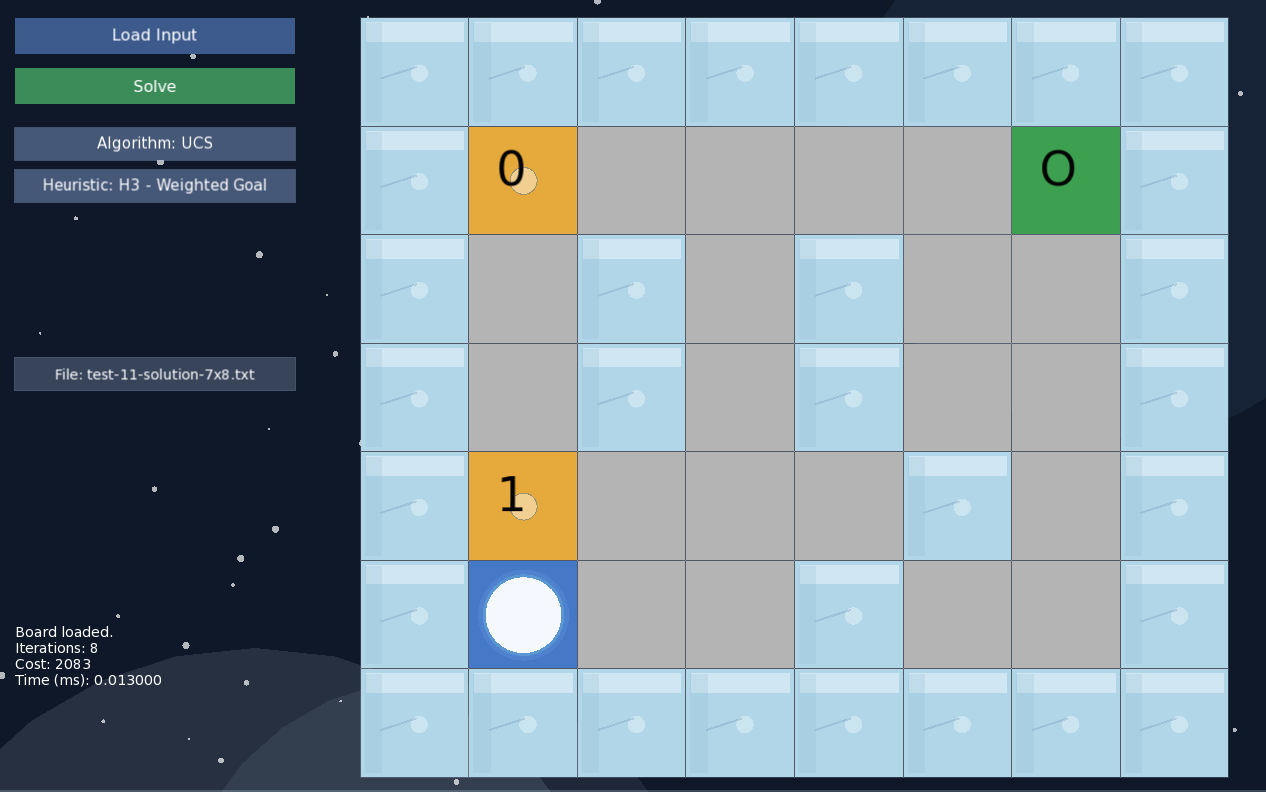
\includegraphics[width=0.25\linewidth]{04-eksperimen/in-4.png} & 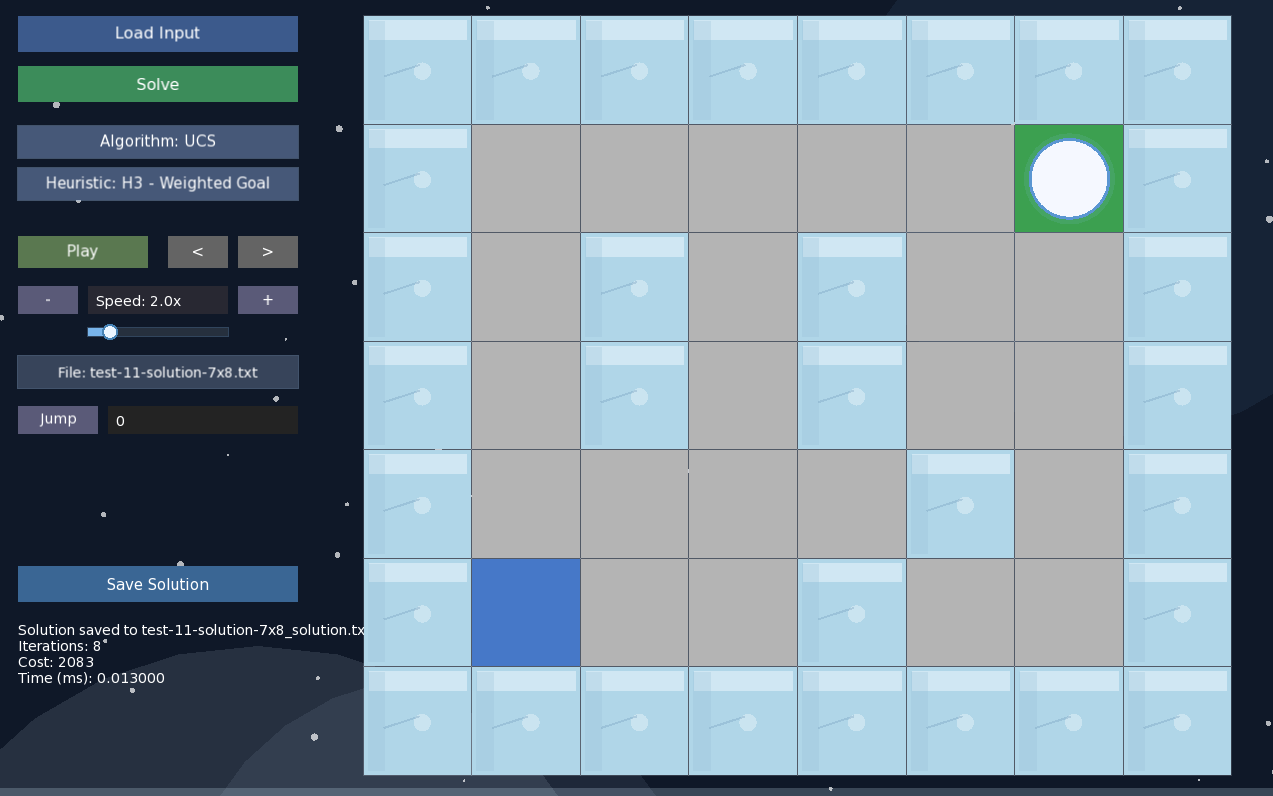
\includegraphics[width=0.25\linewidth]{04-eksperimen/out-4.png} & Test case untuk ukuran $7 \times 8$ dengan Solusi Yang Ditemukan : \texttt{RULDUR} dan Cost dari Solusi : 2083                                     \\

    5  & 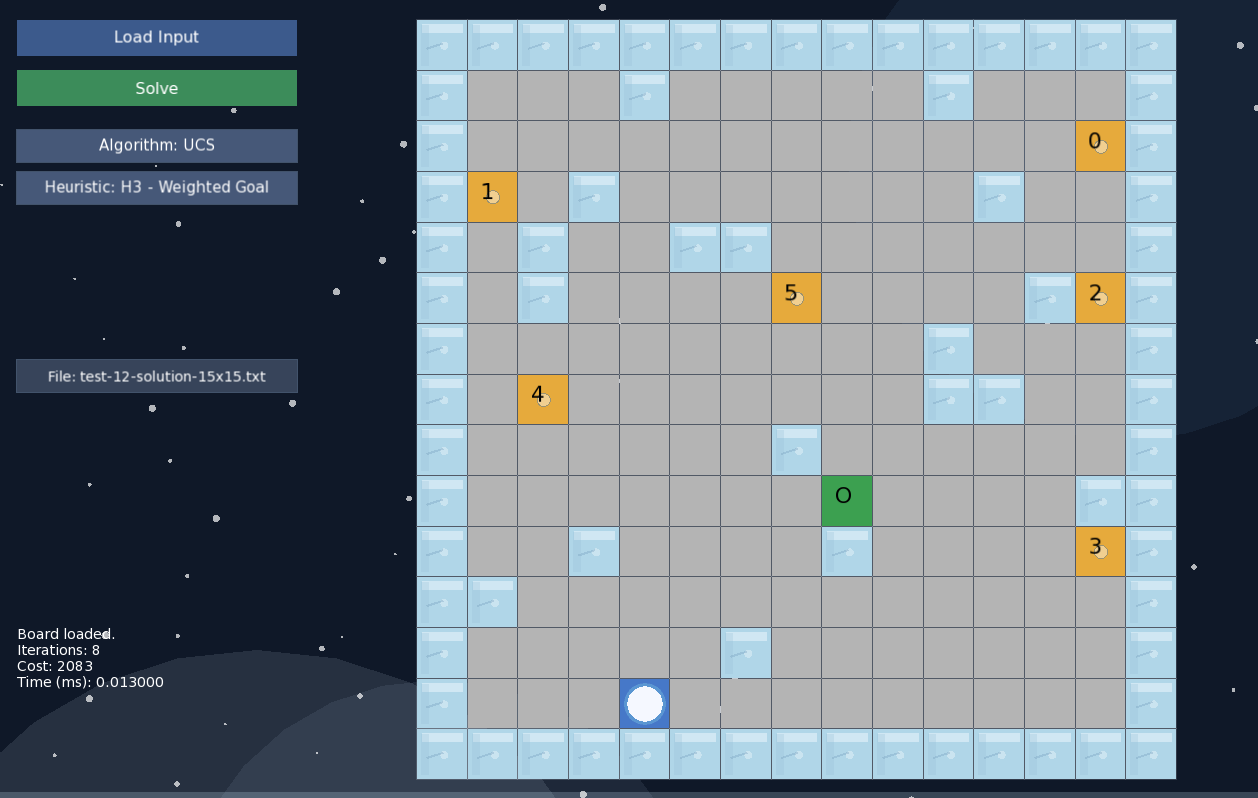
\includegraphics[width=0.25\linewidth]{04-eksperimen/in-5.png} & 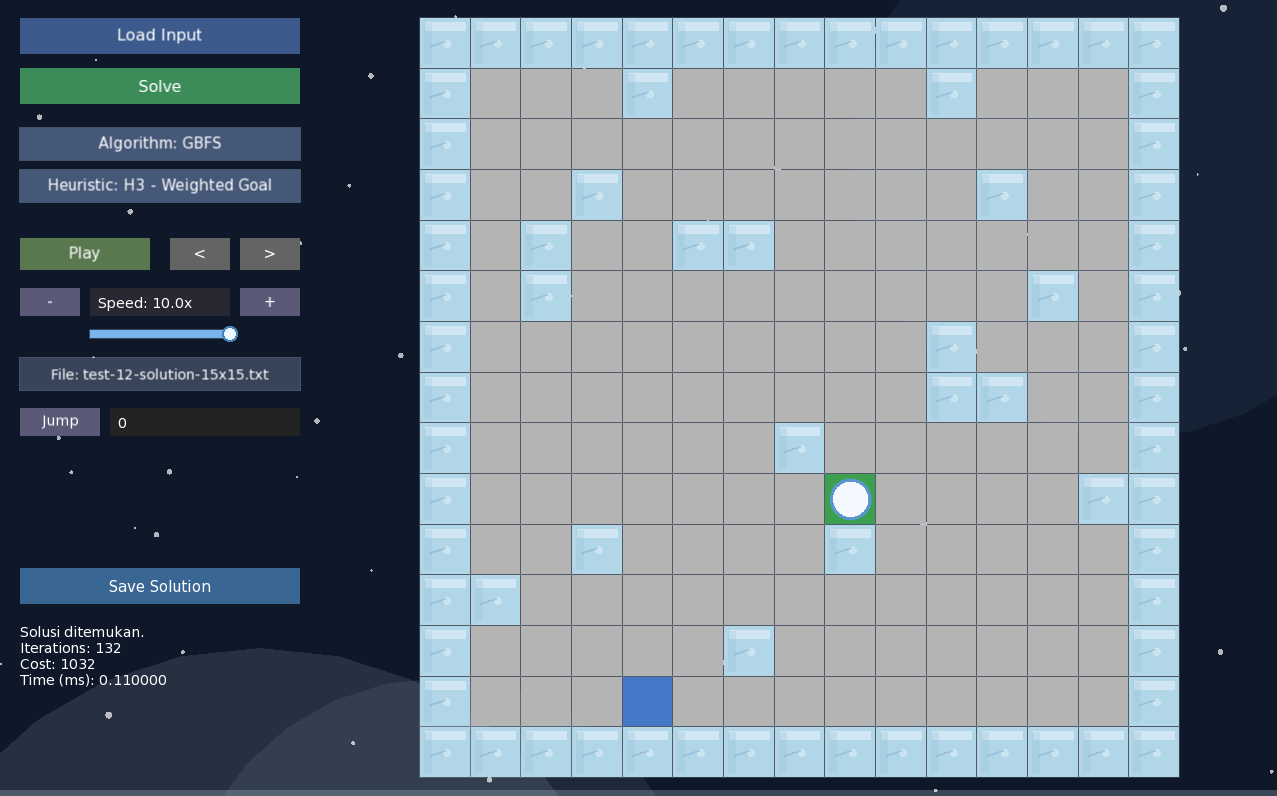
\includegraphics[width=0.25\linewidth]{04-eksperimen/out-5.png} & Test case untuk ukuran $15 \times 15$ dengan Solusi Yang Ditemukan : \texttt{URLDURDRDLURDRULDLURULDLDRURULDRDLRDRDLD} dan Cost dari Solusi : 1026 \\
\end{longtable}

\section{Testing \textit{Edge Cases}}


\begin{longtable}{c c c p{6cm}}
    \caption{Hasil eksperimen: input, output, dan deskripsi}\label{tab:eksperimen}                                                                                                                  \\
    \hline
    No & Gambar Input                                                    & Gambar Output                                                    & Deskripsi                                             \\
    \hline
    \endfirsthead
    \multicolumn{4}{c}{{\bfseries \tablename\ \thetable{} -- lanjutan dari halaman sebelumnya}}                                                                                                     \\
    \hline
    No & Gambar Input                                                    & Gambar Output                                                    & Deskripsi                                             \\
    \hline
    \endhead
    \hline \multicolumn{4}{r}{{Lanjutan pada halaman berikutnya}}                                                                                                                                   \\
    \endfoot
    \hline
    \endlastfoot

    1  & 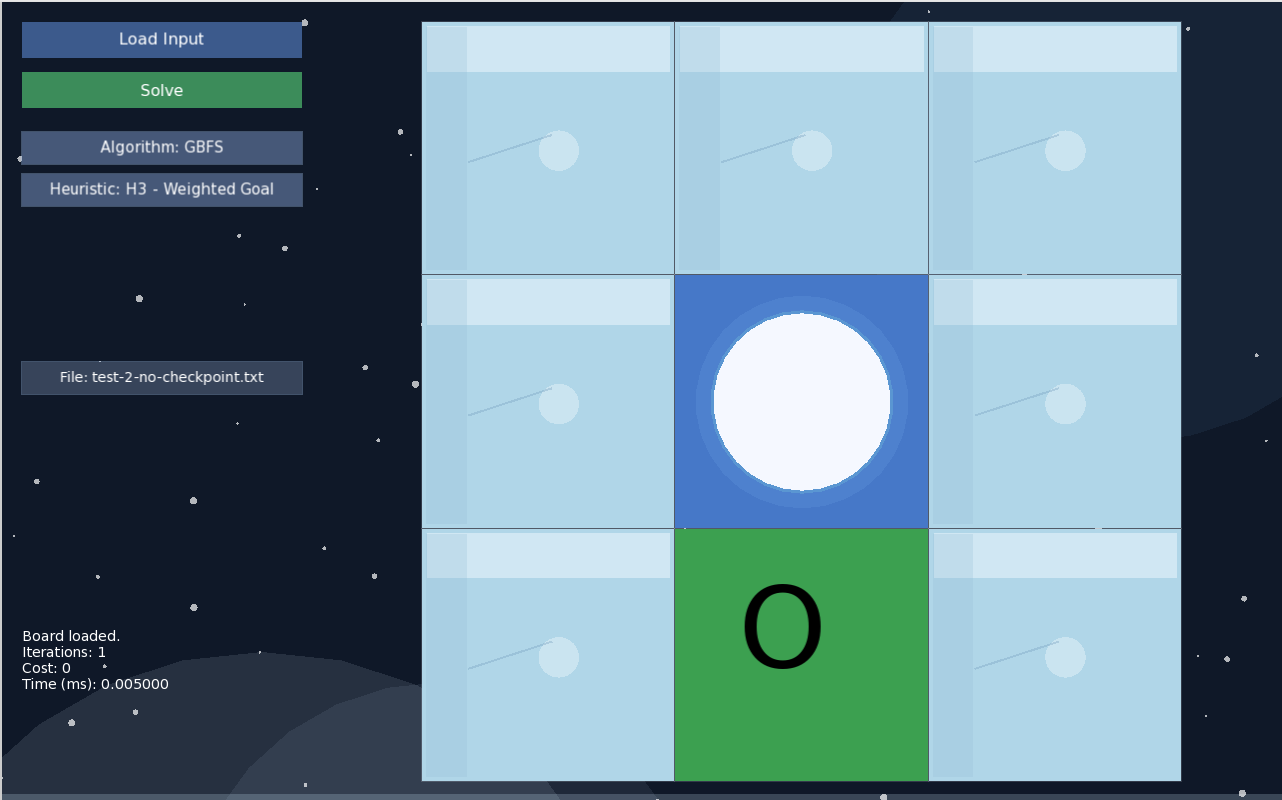
\includegraphics[width=0.25\linewidth]{04-eksperimen/in-6.png}  & 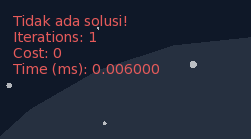
\includegraphics[width=0.25\linewidth]{04-eksperimen/out-6.png}  & Test case pada papan yang tidak memiliki solusi       \\
    2  & 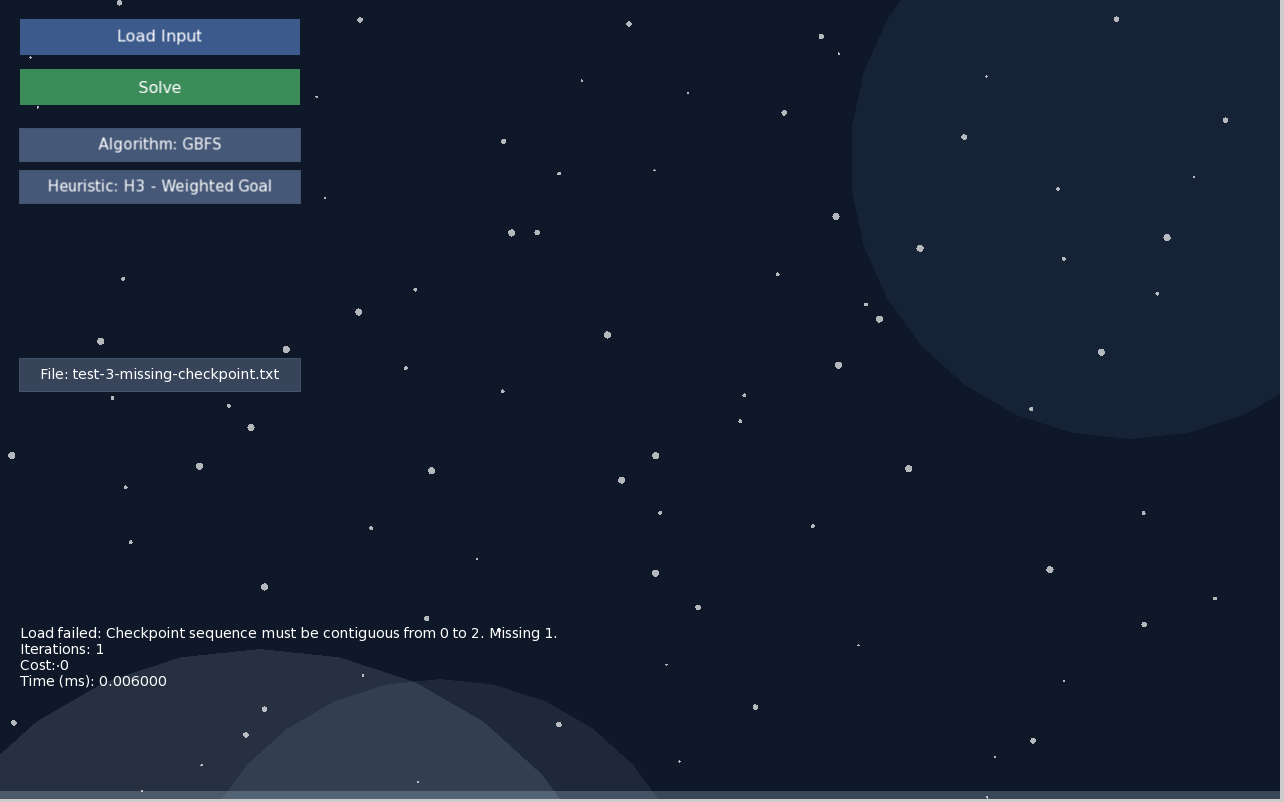
\includegraphics[width=0.25\linewidth]{04-eksperimen/in-7.png}  & 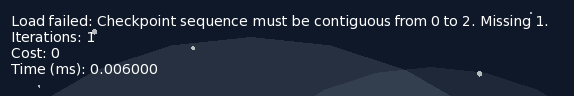
\includegraphics[width=0.25\linewidth]{04-eksperimen/out-7.png}  & Test case dengan papan checkpoint yang tidak kontigu. \\
    3  & 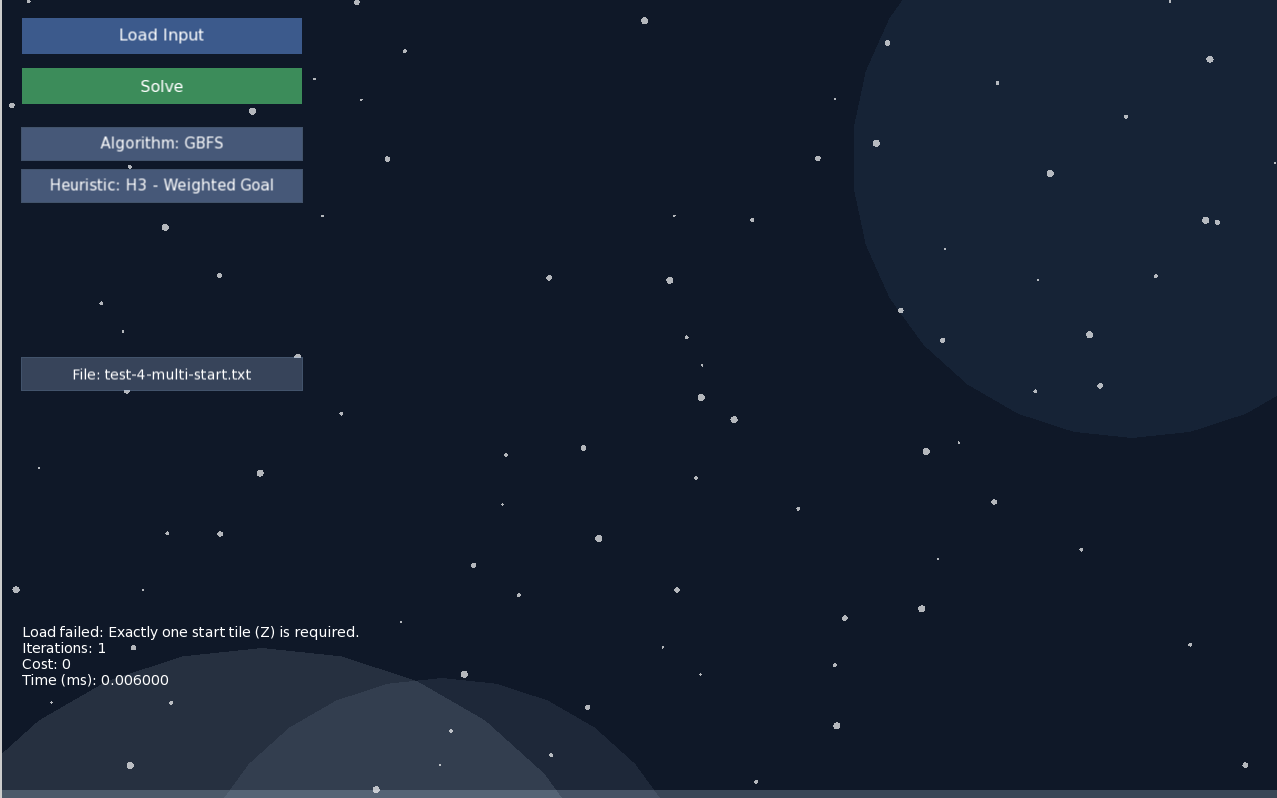
\includegraphics[width=0.25\linewidth]{04-eksperimen/in-8.png}  & 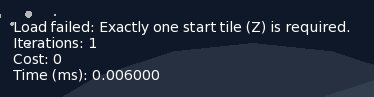
\includegraphics[width=0.25\linewidth]{04-eksperimen/out-8.png}  & Test case dengan papan tidak memiliki titik mulai (Z) \\

    4  & 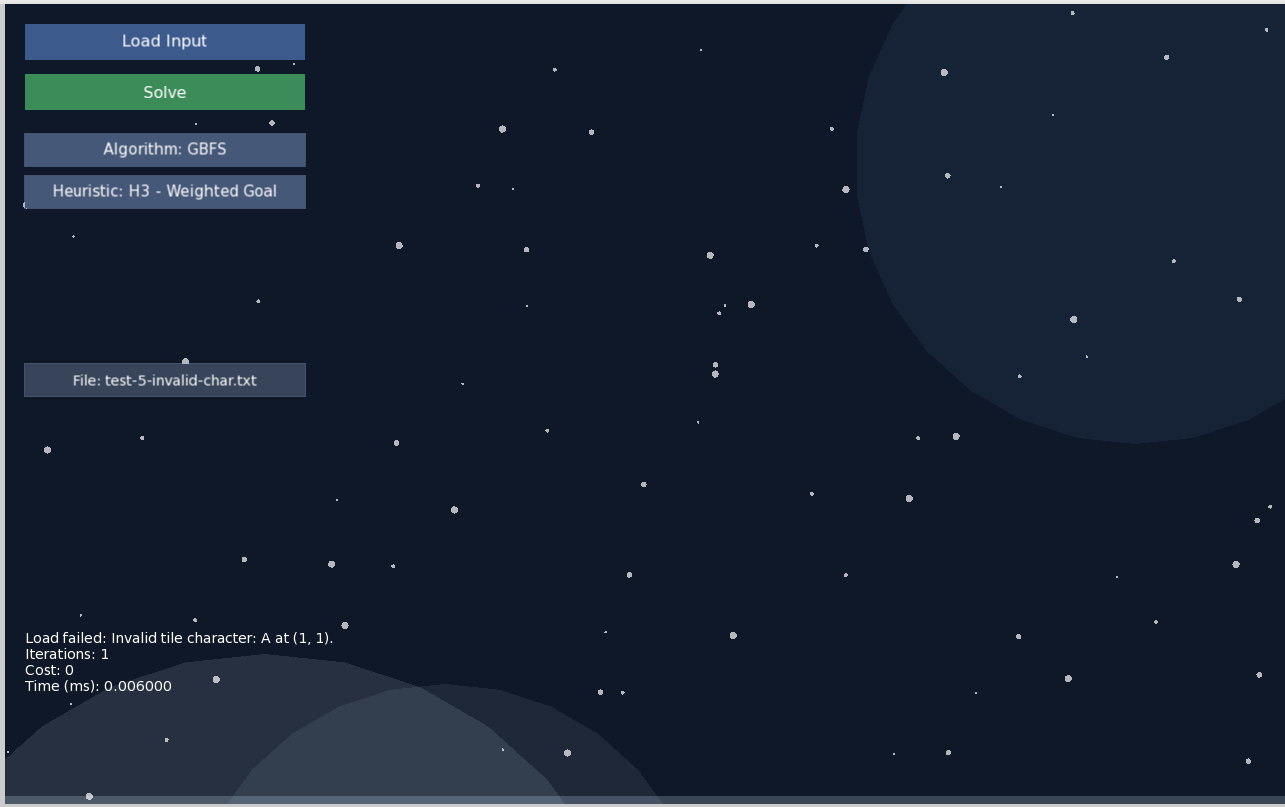
\includegraphics[width=0.25\linewidth]{04-eksperimen/in-9.png}  & 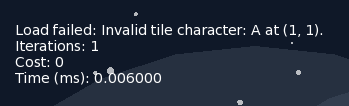
\includegraphics[width=0.25\linewidth]{04-eksperimen/out-9.png}  & Test case untuk papan yang karakternya invalid.       \\

    5  & 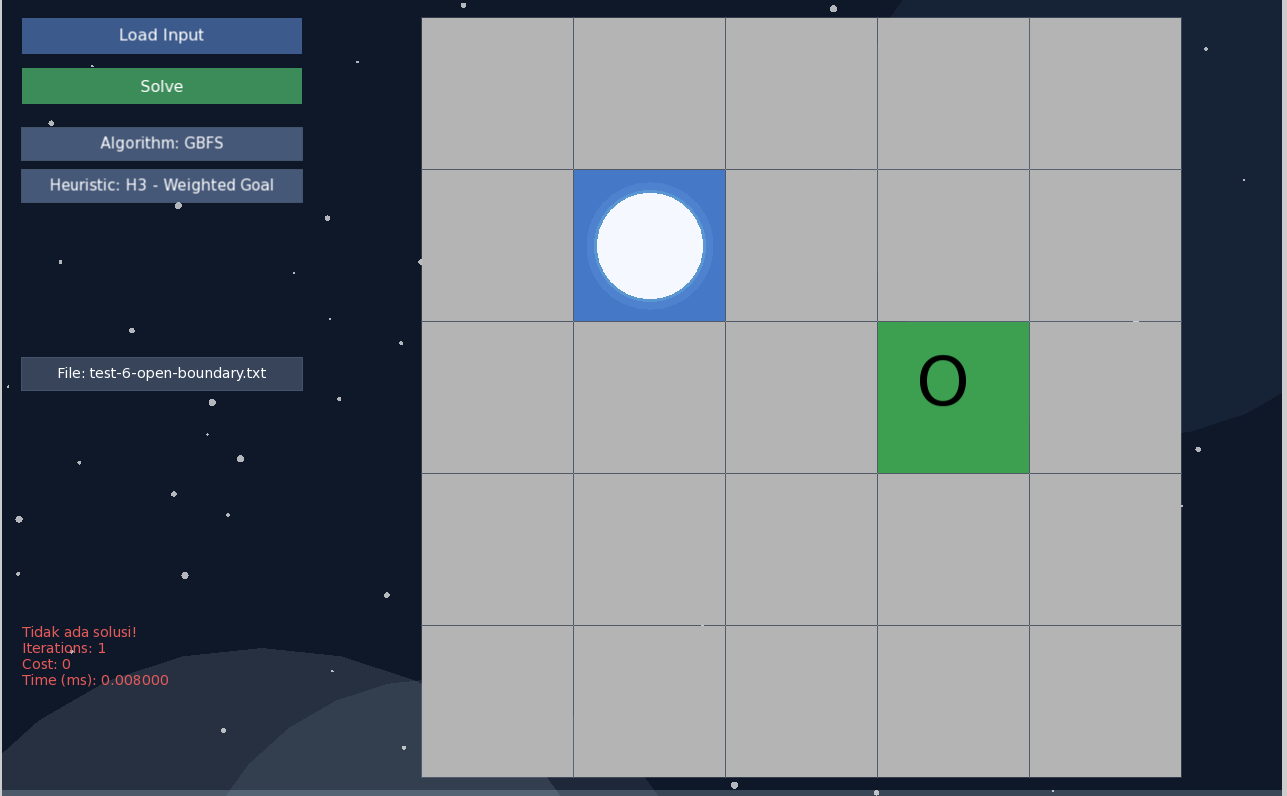
\includegraphics[width=0.25\linewidth]{04-eksperimen/in-10.png} & 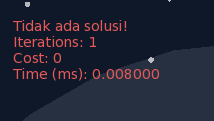
\includegraphics[width=0.25\linewidth]{04-eksperimen/out-10.png} & Test case untuk papan yang tidak punya pembatas.      \\
\end{longtable}


\section{\textit{Post Mortem Analysis}}

\subsection{Pendekatan Algoritma dalam Penyelesaian Masalah}

\subsubsection{Uniform Cost Search (UCS)}

Algoritma UCS menggunakan strategi ekspansi node berdasarkan biaya kumulatif $g(n)$ yang paling rendah. Dalam konteks Ice Sliding Puzzle, setiap node dalam search space merepresentasikan kombinasi dari:
\begin{itemize}
    \item Posisi pin di papan $(row, col)$
    \item Index checkpoint berikutnya yang harus dikunjungi $nextCheckpoint$
\end{itemize}

Pada setiap iterasi, UCS memilih node dengan $g(n)$ terkecil dari priority queue, kemudian mengeksplorasi semua kemungkinan gerak (atas, bawah, kiri, kanan). Untuk setiap gerak, cost dihitung berdasarkan penjumlahan biaya tile yang dilewati selama sliding.

\textbf{Keunggulan:} Menjamin solusi optimal karena ekspansi berdasarkan path cost yang sebenarnya, tanpa heuristik yang mungkin salah.

\textbf{Kelemahan:} Eksplorasi buta tanpa mempertimbangkan jarak ke goal, mengakibatkan banyak node yang tidak perlu dikunjungi.

\subsubsection{Greedy Best-First Search (GBFS)}

GBFS menggunakan strategi ekspansi berdasarkan heuristik $h(n)$ saja, tanpa mempertimbangkan $g(n)$. Algoritma ini memilih node yang paling dekat ke goal berdasarkan estimasi heuristik.

Dalam implementasi, GBFS lebih cepat mencapai goal karena heuristik membimbing pencarian langsung menuju goal, namun tidak menjamin solusi optimal. Eksplorasi dipandu oleh nilai heuristik dengan harapan path yang dieksplorasi lebih sedikit.

\textbf{Keunggulan:} Lebih cepat menemukan solusi pertama karena langsung diarahkan ke goal; memori yang lebih efisien.

\textbf{Kelemahan:} Tidak menjamin solusi optimal; heuristik yang buruk dapat menyebabkan pencarian tersesat.

\subsubsection{A* Search}

A* menggabungkan kedua strategi di atas dengan fungsi evaluasi $f(n) = g(n) + h(n)$. Node yang dipilih adalah yang memiliki $f(n)$ terkecil, menyeimbangkan biaya aktual yang sudah dikeluarkan dengan estimasi sisa biaya menuju goal.

A* lebih optimal dibanding GBFS karena mempertimbangkan path cost, namun lebih efisien dibanding UCS karena menggunakan heuristik untuk membimbing pencarian. Strategi ini dikenal sebagai "informed search" yang sangat efektif untuk problem solving.

\textbf{Keunggulan:} Menjamin solusi optimal jika heuristik bersifat admissible; umumnya lebih cepat daripada UCS.

\textbf{Kelemahan:} Bergantung pada kualitas heuristik; heuristik yang buruk dapat membuat A* tidak lebih efisien dari UCS.

\subsection{Pengaruh Heuristik terhadap Algoritma A* dan GBFS}

Dalam implementasi, terdapat tiga heuristik yang digunakan:

\subsubsection{H1: Manhattan Distance to Target}
Menghitung jarak Manhattan dari posisi sekarang ke target (checkpoint berikutnya atau goal):
$$h_1(n) = |pos.row - target.row| + |pos.col - target.col|$$

Heuristik ini \textbf{admissible} karena jarak Manhattan selalu kurang dari atau sama dengan jarak sebenarnya pada grid dengan pergerakan 4-arah. Sangat efektif untuk papan kecil hingga menengah dengan banyak checkpoint.

\subsubsection{H2: Remaining Checkpoints + Manhattan}
Mengkombinasikan jumlah checkpoint yang belum dikunjungi dengan jarak Manhattan ke target berikutnya:
$$h_2(n) = (\text{maxCheckpoint} - \text{nextCheckpoint}) + \text{manhattan}(pos, target)$$

Heuristik ini \textbf{tidak admissible} pada beberapa kasus karena menjumlahkan komponen yang mungkin over-estimate jarak sebenarnya. Namun, memberikan penghargaan lebih tinggi pada state yang sudah melewati banyak checkpoint, memprioritaskan path yang progresif menuju goal.

\subsubsection{H3: Weighted Remaining to Goal}
Memberikan bobot pada checkpoint sisa dengan faktor 2, ditambah jarak Manhattan ke goal akhir:
$$h_3(n) = \text{manhattan}(pos, goal) + 2 \times (\text{maxCheckpoint} - \text{nextCheckpoint})$$

Heuristik ini juga \textbf{tidak admissible} karena bobot 2 dapat menyebabkan over-estimation. Namun, sangat berguna untuk mencegah algoritma terjebak mengeksplorasi branch dengan sedikit checkpoint.

\textbf{Observasi:} H2 dan H3 yang non-admissible tetap berguna dalam praktik karena mempercepat pencarian meskipun tidak menjamin optimalitas. A* dengan H2 atau H3 masih menemukan solusi valid, hanya tidak dijamin optimal.

\subsection{Kasus Kegagalan Tiap Algoritma}

\subsubsection{Kasus Kegagalan UCS}
\begin{itemize}
    \item \textbf{Papan besar tanpa struktur jelas:} UCS akan mengeksplorasi banyak node karena tidak memiliki petunjuk arah goal. Pada papan $15 \times 15$, jumlah iterasi dapat mencapai ribuan bahkan untuk kasus sederhana.
    \item \textbf{Waktu eksekusi lama:} Tanpa heuristik, UCS tidak dapat membedakan antara path yang menjanjikan dan path yang sia-sia.
\end{itemize}

\subsubsection{Kasus Kegagalan GBFS}
\begin{itemize}
    \item \textbf{Heuristik yang menyesatkan:} Jika heuristik terlalu optimistis atau tidak selaras dengan struktur problem, GBFS dapat terjebak di local minimum. Contoh: jika ada rintangan besar antara posisi dan goal, GBFS mungkin tetap mengejar path langsung meskipun tidak valid.
    \item \textbf{Solusi sub-optimal:} GBFS dapat menemukan solusi pertama dengan cost lebih tinggi daripada solusi optimal.
    \item \textbf{Papan dengan banyak checkpoint:} Heuristik yang hanya melihat checkpoint berikutnya tanpa memperhitungkan sisa checkpoint dapat menyebabkan eksplorasi tidak efisien.
\end{itemize}

\subsubsection{Kasus Kegagalan A*}
\begin{itemize}
    \item \textbf{Heuristik non-admissible yang buruk:} Meskipun jarang, heuristik yang over-estimate terlalu jauh dapat menyebabkan A* melewatkan solusi optimal dan berhenti di solusi sub-optimal.
    \item \textbf{Memory overhead:} Pada papan besar, A* dapat menggunakan banyak memori untuk menyimpan open set dan closed set, terutama jika search space sangat besar.
    \item \textbf{Tidak ada solusi:} Jika papan tidak memiliki jalur valid menuju goal (misalnya checkpoint tidak terjangkau atau terhalang), ketiga algoritma akan gagal menemukan solusi. Dalam implementasi, program mendeteksi dan melaporkan "Solusi tidak ditemukan."
\end{itemize}

\subsection{Kesimpulan Observasi}

Dari hasil eksperimen, observasi berikut dapat dibuat:
\begin{itemize}
    \item \textbf{UCS vs A*:} A* dengan H1 umumnya lebih cepat 2--5x lipat dibanding UCS pada papan besar, dengan hasil solusi yang sama (optimal).
    \item \textbf{GBFS vs A*:} GBFS paling cepat namun dapat menghasilkan solusi sub-optimal; A* lebih lambat dari GBFS tetapi menjamin optimalitas.
    \item \textbf{Pengaruh Heuristik:} H1 (Manhattan murni) lebih konsisten dan admissible; H2 dan H3 lebih agresif namun risiko sub-optimal lebih tinggi.
    \item \textbf{Scalability:} Ketiga algoritma dapat diterapkan pada papan hingga $15 \times 15$ dalam waktu masuk akal (< 1 detik). Untuk papan lebih besar, optimasi tambahan mungkin diperlukan.
\end{itemize}

\chapter{Penutup}
Tugas ini disusun sepenuhnya tanpa bantuan kecerdasan buatan (Generative AI),
melainkan hasil pemikiran dan analisis mandiri.

\begin{flushright}
    Bandung, 25 Maret 2026
    \vspace{3px}

    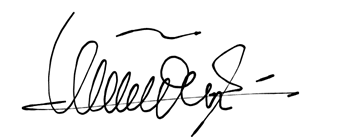
\includegraphics[width=0.4\textwidth]{ttd-aufar.png}

    \vspace{3px}
    Muhammad Aufar Rizqi Kusuma\\
    13524061
\end{flushright}

\chapter{Lampiran}
\section{Tautan GitHub}
\href{https://github.com/parkuskus/Tucil3_13524061}{Link GitHub}

\section{Checklist Tucil}

\begin{table}[H]
    \centering
    \renewcommand{\arraystretch}{1.2}
    \begin{tabular}{|c|p{9cm}|c|c|}
        \hline
        No & Poin                                                              & Ya           & Tidak        \\
        \hline
        1  & Program berhasil dikompilasi tanpa kesalahan                      & $\checkmark$ & $\square$    \\
        \hline
        2  & Program berhasil dijalankan                                       & $\checkmark$ & $\square$    \\
        \hline
        3  & Solusi benar dan mematuhi aturan permainan                        & $\checkmark$ & $\square$    \\
        \hline
        4  & Dapat membaca \texttt{.txt} dan menyimpan solusi ke \texttt{.txt} & $\checkmark$ & $\square$    \\
        \hline
        5  & Memiliki GUI                                                      & $\checkmark$ & $\square$    \\
        \hline
        6  & Ada algoritma pathfinding alternatif                              & $\square$    & $\checkmark$ \\
        \hline
        7  & Ada dua heuristik alternatif tambahan                             & $\checkmark$ & $\square$    \\
        \hline
    \end{tabular}
\end{table}


\nocite{*}
\bibliography{dafpus}


\end{document}
